\documentclass[a4paper,14pt]{extreport}

\usepackage[left=20mm,right=20mm,top=20mm,bottom=20mm]{geometry}
\usepackage{fontspec}
\usepackage{microtype}
\usepackage{polyglossia}
\usepackage{tabularx}
\setmainlanguage{russian}

\setmainfont{Times Newer Roman}[Ligatures=TeX]
\newfontfamily\cyrillicfont{Times Newer Roman}[Ligatures=TeX]
\setsansfont{Liberation Sans}
\setmonofont{Liberation Mono}
\newfontfamily\cyrillicfontsf{Liberation Sans}
\newfontfamily\cyrillicfonttt{Liberation Mono}

\renewcommand\normalsize{\fontsize{14pt}{21pt}\selectfont}
\renewcommand\small{\fontsize{12pt}{18pt}\selectfont}
\renewcommand\large{\fontsize{16pt}{24pt}\selectfont}
\renewcommand\Large{\fontsize{18pt}{27pt}\selectfont}
\renewcommand\LARGE{\fontsize{20pt}{30pt}\selectfont}

\usepackage{usm-title}

\authorname{Анисимов Виктор}
\thesistitle{Автономная операционная система самооптимизации и самолечения}
\speciality{ПРИКЛАДНАЯ ИНФОРМАТИКА}
\group{IA2403}
\supervisor{Croitor Mihail}
\departmenthead{Capcelea Titu, doctor, conferențiar universitar}
\yearofdefense{2026}

\usepackage{tocloft}
\usepackage{chngcntr}
\usepackage{titlesec}
\renewcommand{\thesection}{\Roman{section}}
\counterwithin{subsection}{section}
\renewcommand{\thesubsection}{\arabic{section}.\arabic{subsection}}
\counterwithin{subsubsection}{subsection}
\renewcommand{\thesubsubsection}{\thesubsection.\arabic{subsubsection}}
\titleformat{\section}[block]
  {\normalfont\Large\bfseries\centering}
  {\thesection}
  {1em}
  {}
\titleformat{name=\section,numberless}[block]
  {\normalfont\Large\bfseries\centering}
  {}
  {0pt}
  {}
\setcounter{tocdepth}{3}
\setcounter{secnumdepth}{3}
\renewcommand{\cfttoctitlefont}{\hfill\bfseries}
\renewcommand{\cftaftertoctitle}{\hfill\hfill}
\renewcommand{\cftsecfont}{\normalfont\bfseries}
\renewcommand{\cftsecpagefont}{\normalfont\bfseries}

\usepackage{etoolbox}
\gappto\captionsrussian{\renewcommand{\contentsname}{СОДЕРЖАНИЕ}}
\makeatletter
\renewenvironment{thebibliography}[1]
     {\list{\@biblabel{\@arabic\c@enumiv}}%
           {\settowidth\labelwidth{\@biblabel{#1}}%
            \leftmargin\labelwidth
            \advance\leftmargin\labelsep
            \@openbib@code
            \usecounter{enumiv}%
            \let\p@enumiv\@empty
            \renewcommand\theenumiv{\@arabic\c@enumiv}}%
      \sloppy\clubpenalty4000\widowpenalty4000%
      \sfcode`\.\@m}
     {\def\@noitemerr
       {\@latex@warning{Empty `thebibliography' environment}}%
      \endlist}
\makeatother

\usepackage{xurl}
\usepackage{hyperref}
\hypersetup{hidelinks}
\usepackage{xcolor}
\definecolor{codebg}{HTML}{F7F7F7}
\definecolor{codeframe}{HTML}{B8B8B8}
\usepackage{caption}
\usepackage{float}
\usepackage[newfloat]{minted}
\SetupFloatingEnvironment{listing}{name=Листинг}
\setminted{
  bgcolor=codebg,
  breaklines=true,
  frame=lines,
  framesep=6pt,
  framerule=0.4pt,
  fontsize=\small,
  linenos=true,
  numbersep=8pt,
  rulecolor=codeframe,
  tabsize=2
}
\usepackage{tabularx}
\usepackage{longtable}
\usepackage{booktabs}
\usepackage{array}
\usepackage{graphicx}
\usepackage{amsmath}
\usepackage{amssymb}
\usepackage{mathtools}
\emergencystretch=4em
\tolerance=2000
\hbadness=3000

\begin{document}

\maketitlepage
\tableofcontents

\clearpage
\section*{СПИСОК ПРИНЯТЫХ СОКРАЩЕНИЙ}
\addcontentsline{toc}{section}{СПИСОК ПРИНЯТЫХ СОКРАЩЕНИЙ}
\begin{longtable}{p{0.18\textwidth}p{0.72\textwidth}}
\toprule
Сокращение & Расшифровка \\
\midrule
GA & Генетический алгоритм (Genetic Algorithm) \\
SA & Имитация отжига (Simulated Annealing) \\
TS & Поиск с запретами (Tabu Search) \\
CP-SAT & Constraint Programming — Satisfiability (решатель ограничений на основе SAT, Google OR-Tools) \\
СУБД    & Система управления базами данных \\
БД      & База данных |
API     & Application Programming Interface (программный интерфейс) \\
NP      & Класс задач недетерминированной полиномиальной сложности \\
ООП     & Объектно-ориентированное программирование \\
ORM     & Object-Relational Mapping (объектно-реляционное отображение) \\
\bottomrule
\end{longtable}


\clearpage
\section*{ВВЕДЕНИЕ}
\addcontentsline{toc}{section}{ВВЕДЕНИЕ}
# Введение

Составление расписания занятий — одна из тех задач университетской жизни, которая кажется простой ровно до тех пор, пока не приходится решать её на практике. На первый взгляд нужно всего лишь расставить пары так, чтобы преподаватель не оказался одновременно в двух аудиториях, а группа не получила две дисциплины в одно и то же время. Но как только в задачу добавляются реальные ограничения — вместимость аудиторий, специализация кабинетов под лабораторные работы, нагрузка преподавателей, желание не растягивать день большими окнами между парами — простая на словах задача превращается в комбинаторную головоломку, ручное решение которой занимает у методистов вуза дни, а иногда недели в начале каждого семестра.

Это не локальная проблема одного учебного заведения. Задача составления расписания относится к классу NP-трудных задач: с ростом числа дисциплин, групп, преподавателей и аудиторий количество возможных вариантов расписания растёт настолько быстро, что полный перебор всех вариантов перестаёт быть осуществимым на практике уже при умеренных объёмах данных. Это делает задачу интересной не только с практической, но и с алгоритмической точки зрения: она оказывается удобным полигоном для сравнения разных подходов к решению NP-трудных задач — от точных методов до эвристик, не гарантирующих оптимальность, но способных найти хорошее решение за разумное время.

Актуальность темы для практики очевидна: автоматизация составления расписания напрямую экономит время методистов и снижает число ошибок, неизбежных при ручной расстановке сотен пар. Актуальность для учебной и исследовательской работы — в том, что задача составления расписания одновременно простая для понимания (любой человек интуитивно понимает условия и ограничения) и достаточно сложная, чтобы на ней можно было содержательно сравнить разные алгоритмические парадигмы: эволюционные методы, методы локального поиска, точное программирование ограничений. Это даёт возможность не просто реализовать один алгоритм, а провести осмысленное сравнение нескольких принципиально разных подходов на одной и той же постановке задачи.

Целью данной работы является разработка и сравнительный анализ нескольких алгоритмов автоматического построения расписания учебных занятий, способных учитывать как обязательные (жёсткие), так и желательные (мягкие) ограничения, присущие реальному учебному процессу.

Для достижения этой цели были поставлены следующие задачи:

Во-первых, изучить теоретические основы задачи составления расписания и существующие подходы к её решению, чтобы выбрать алгоритмы, наиболее подходящие для рассматриваемой постановки задачи. Во-вторых, спроектировать единую модель данных и единый критерий оценки качества расписания, на основе которых можно реализовать и затем честно сравнить между собой разные алгоритмы. В-третьих, реализовать четыре алгоритма построения расписания — генетический алгоритм, имитацию отжига, поиск с запретами и программирование ограничений (CP-SAT) — на основе этой единой модели. В-четвёртых, провести экспериментальное сравнение реализованных алгоритмов по нескольким критериям: качество найденного решения, скорость работы, устойчивость к разной структуре исходных данных. В-пятых, сформулировать практические выводы о применимости каждого из подходов в зависимости от размера и характера задачи.

Методологическую базу работы составили анализ научной и технической литературы по теории расписаний и методам комбинаторной оптимизации, проектирование и реализация программного обеспечения на языке Python с использованием библиотек DEAP (генетические алгоритмы) и OR-Tools (CP-SAT), а также вычислительный эксперимент: серия прогонов всех четырёх алгоритмов на синтетических наборах данных различного размера и сложности с последующим статистическим сравнением результатов.

Работа состоит из трёх глав. В первой главе рассматриваются теоретические основы задачи составления расписания: формальная постановка задачи, понятие жёстких и мягких ограничений, а также краткий обзор существующих программных решений в этой области. Во второй главе подробно описывается каждый из четырёх реализованных алгоритмов — принципы его работы, особенности конкретной реализации, проблемы, возникшие в процессе разработки, и выводы по применимости каждого алгоритма, — а также приводится сравнительный анализ всех четырёх подходов по результатам вычислительного эксперимента. В заключении подводятся итоги проделанной работы и обозначаются возможные направления её дальнейшего развития.


\clearpage
\section{ПРОБЛЕМА СОСТАВЛЕНИЯ РАСПИСАНИЯ}
# I.1. Теория составления расписания
\subsection{Теория составления расписания}
В формальной постановке задача составления расписания (timetabling problem) сводится к распределению конечного набора событий — учебных занятий — по конечному набору ресурсов: моментов времени, аудиторий и преподавателей, при соблюдении заданного набора ограничений. Несмотря на кажущуюся простоту формулировки, задача относится к классу NP-трудных: уже при умеренном числе дисциплин, групп и аудиторий пространство возможных расписаний исчисляется величинами порядка десятков и сотен порядков, что делает полный перебор всех вариантов принципиально неприменимым на практике. Этот факт — отправная точка для всего дальнейшего изложения: именно невозможность гарантированно быстро найти оптимальное решение методом перебора и заставляет применять либо точные методы с отсечением пространства поиска (программирование ограничений), либо эвристические методы, не гарантирующие оптимальность, но способные найти приемлемое решение за разумное время (генетические алгоритмы, имитация отжига, поиск с запретами).

Ограничения, накладываемые на расписание, принято делить на две категории.
\begin{itemize}
\item Жёсткие ограничения (hard constraints) — это условия, нарушение которых делает расписание физически нереализуемым: преподаватель не может одновременно вести два занятия, аудитория не может одновременно использоваться двумя группами, число пар в день не может превышать вместимость учебной сетки. Расписание, нарушающее хотя бы одно жёсткое ограничение, считается недопустимым (infeasible) независимо от того, насколько хорошо оно удовлетворяет остальным критериям. 
\item Мягкие ограничения (soft constraints), напротив, описывают желательные, но не обязательные свойства расписания: компактность занятий в течение дня без больших окон, соответствие вместимости аудитории размеру группы, равномерное распределение нагрузки по дням недели. Нарушение мягкого ограничения не делает расписание недопустимым, но снижает его качество. 
\end{itemize}

Эта классификация — жёсткие ограничения как фильтр допустимости, мягкие как критерий качества среди допустимых решений — лежит в основе практически всех современных подходов к автоматизации составления расписаний и используется как сквозная идея во второй главе настоящей работы при описании каждого из реализованных алгоритмов.

Исторически задачи такого типа решались методами целочисленного линейного программирования, позже — методами локального поиска и метаэвристиками, заимствованными из теории эволюционных вычислений и статистической физики. Появление современных решателей задач выполнимости ограничений (constraint satisfaction) и, в частности, гибридных SAT-решателей вернуло интерес к точным методам, способным не просто находить решение, но и доказывать его оптимальность либо отсутствие решения вовсе. Именно это разнообразие — от точных методов до чисто эвристических — определило выбор четырёх алгоритмов, рассматриваемых в данной работе, и стало основанием для их сравнительного анализа.


\subsection{Анализ существующих инструментов}

Существующие программные решения для автоматизации составления расписания можно условно разделить на три группы. Первая — это узкоспециализированные коммерческие и открытые системы вузовского масштаба (например, системы класса ASC Timetables, FET — Free Timetabling Software, и аналогичные отечественные разработки), ориентированные на конечного пользователя — методиста, который задаёт исходные данные через графический интерфейс и получает готовое расписание без необходимости разбираться в алгоритмической стороне вопроса. Такие системы, как правило, используют один конкретный алгоритм (чаще всего метаэвристику — генетический алгоритм либо локальный поиск) и не предоставляют возможности сравнить его с альтернативными подходами на тех же данных, поскольку это не входит в задачи конечного продукта.

Вторая группа — это академические и исследовательские реализации, публикуемые в рамках научных работ по теории расписаний; именно из этого пласта литературы заимствована классификация ограничений на жёсткие и мягкие, рассмотренная в предыдущем разделе, а также большинство идей, реализованных во второй главе настоящей работы (атрибутный табу-лист, критерий Метрополиса, индексное кодирование решения для генетических алгоритмов). Такие работы, как правило, сосредоточены на одном алгоритме и его модификациях, а не на сравнении принципиально разных парадигм.

Третья группа — это общие библиотеки и решатели для задач комбинаторной оптимизации, не привязанные к предметной области расписаний напрямую: библиотека DEAP для эволюционных вычислений на Python, решатель ограничений CP-SAT в составе Google OR-Tools, а также универсальные методы глобальной оптимизации (например, имитация отжига в составе библиотеки SciPy). Эти инструменты избавляют от необходимости реализовывать базовые механизмы алгоритмов с нуля, но требуют адаптации к конкретной предметной области: большинство таких библиотек спроектированы для непрерывных или слабо структурированных задач, и применение их «как есть» к задаче расписания с дискретными, категориальными переменными (номер аудитории, идентификатор преподавателя) требует существенной переработки представления решения и операторов поиска — этот вопрос подробно разбирается в начале каждой подглавы второй главы при описании конкретной реализации.

Общий недостаток существующих решений всех трёх групп — отсутствие единой, воспроизводимой методики сравнения разных алгоритмов на одной и той же постановке задачи. Коммерческие системы скрывают алгоритмическую кухню от пользователя, академические работы сравнивают модификации одного алгоритма между собой, а универсальные библиотеки предоставляют инструменты, но не готовую методологию сравнения. Именно эта пробел и определяет практическую направленность второй главы настоящей работы: реализовать несколько принципиально разных алгоритмов на единой модели данных, с единым критерием оценки качества решения, и провести их сравнение на одинаковых наборах исходных данных.


\clearpage
\section{АЛГОРИТМЫ СОСТАВЛЕНИЯ РАСПИСАНИЯ}
\subsection{Генетический алгоритм. (Genetic Algorithm)}
\input{sections/GA}
\subsection{Имитация отжига(Simulated Annealing)}
 
\subsubsection{ Общие принципы и введение в алгоритм}

Имитация отжига — метод локального поиска, заимствующий аналогию из металлургии: при медленном охлаждении металла его атомы успевают занять состояние с минимальной энергией, тогда как быстрое охлаждение «замораживает» металл в случайном, не обязательно наилучшем состоянии. В применении к оптимизации это означает следующее: алгоритм работает с одним текущим решением и на каждом шаге пробует случайное небольшое изменение этого решения (один «ход»). Если изменение улучшает решение, оно принимается всегда. Если изменение ухудшает решение, оно всё равно может быть принято — но с вероятностью, которая убывает по мере того, как убывает управляющий параметр алгоритма, называемый температурой. На старте, при высокой температуре, алгоритм почти всегда соглашается на ухудшающие ходы, что позволяет ему свободно перемещаться по пространству решений и не застревать в первом найденном локальном оптимуме. По мере охлаждения вероятность принять ухудшение падает, и к концу работы алгоритм ведёт себя как обычный жадный локальный поиск, только уже отталкиваясь от гораздо более удачной стартовой точки, чем в начале.

При выборе инструмента для реализации имитации отжига изначально рассматривался готовый решатель scipy.optimize.dual_annealing — однако его применение к задаче расписания было признано нецелесообразным и впоследствии заменено самостоятельной реализацией. Причина в том, что dual_annealing, как и большинство готовых реализаций имитации отжига в общих научных библиотеках, спроектирован для задач с непрерывными переменными в заданных границах: представление решения в нём — это вектор вещественных чисел, а не дискретный набор категориальных решений (номер аудитории, идентификатор преподавателя). Применение такого решателя к дискретной задаче требовало бы искусственного округления вещественных координат до целочисленных индексов внутри функции оценки качества, что превращает функцию оценки в кусочно-постоянную и обесценивает встроенный в решатель механизм локальной градиентной доводки решения, рассчитанный на гладкие функции. Вместо этого был реализован классический дискретный вариант имитации отжига, работающий непосредственно с теми же дискретными ходами (изменение дня и пары занятия, замена аудитории, замена преподавателя, обмен временными слотами между двумя занятиями), что и в поиске с запретами, описанном в следующем разделе — но принципиально иначе использующий эти ходы: без памяти о предыдущих состояниях и с вероятностным, а не детерминированным критерием принятия.

\subsubsection{ Особенности реализации}

Каждая итерация алгоритма генерирует ровно один случайный ход и применяет его непосредственно к текущему расписанию, не создавая его копию — в отличие от поиска с запретами, где на каждой итерации оценивается целый пакет ходов-кандидатов. Это решение продиктовано тем, что имитация отжига обычно требует существенно большего числа итераций для полноценного прохождения цикла охлаждения, и копирование всего расписания на каждую (в большинстве случаев — отклонённую) попытку оказалось бы неоправданно расточительным. Вместо копирования реализован явный механизм отмены хода: каждая функция применения хода возвращает прежнее значение изменённого элемента расписания, и в случае отказа от хода это прежнее значение возвращается на место.

\captionof{listing}{Логика принятия и отклонения шага}
\begin{minted}{python}
delta = energy(candidate) - energy(current)
if delta <= 0 or random() < exp(-delta / temperature):
    accept_move()
else:
    revert_move()
temperature *= cooling_rate
\end{minted}

Отдельного внимания заслуживает то, что критерий принятия хода и критерий отбора лучшего из найденных решений за всю историю работы реализованы по-разному и намеренно не смешаны между собой. Для критерия принятия пара чисел «нарушения жёстких ограничений, штраф по мягким ограничениям» сводится к одному вещественному числу — иначе формула вероятности принятия, требующая единственного числового значения разницы энергий, была бы неприменима. Но при отборе лучшего решения за всю историю поиска используется точное сравнение исходной пары чисел без сведения к одному значению, поскольку именно так сохраняется строгий приоритет допустимости расписания над его мягким качеством.

\subsubsection{ Метрики

\paragraph {Динамика поиска}

Алгоритм демонстрирует выраженный стохастический характер сходимости. На ранних этапах поиска наблюдается значительный «шум» вследствие принятия решений об ухудшении целевой функции, что позволяет алгоритму покидать локальные оптимумы. По мере снижения температуры (остывания) график сходимости приобретает плавный нисходящий характер.

\begin{figure}[h]
    \centering
    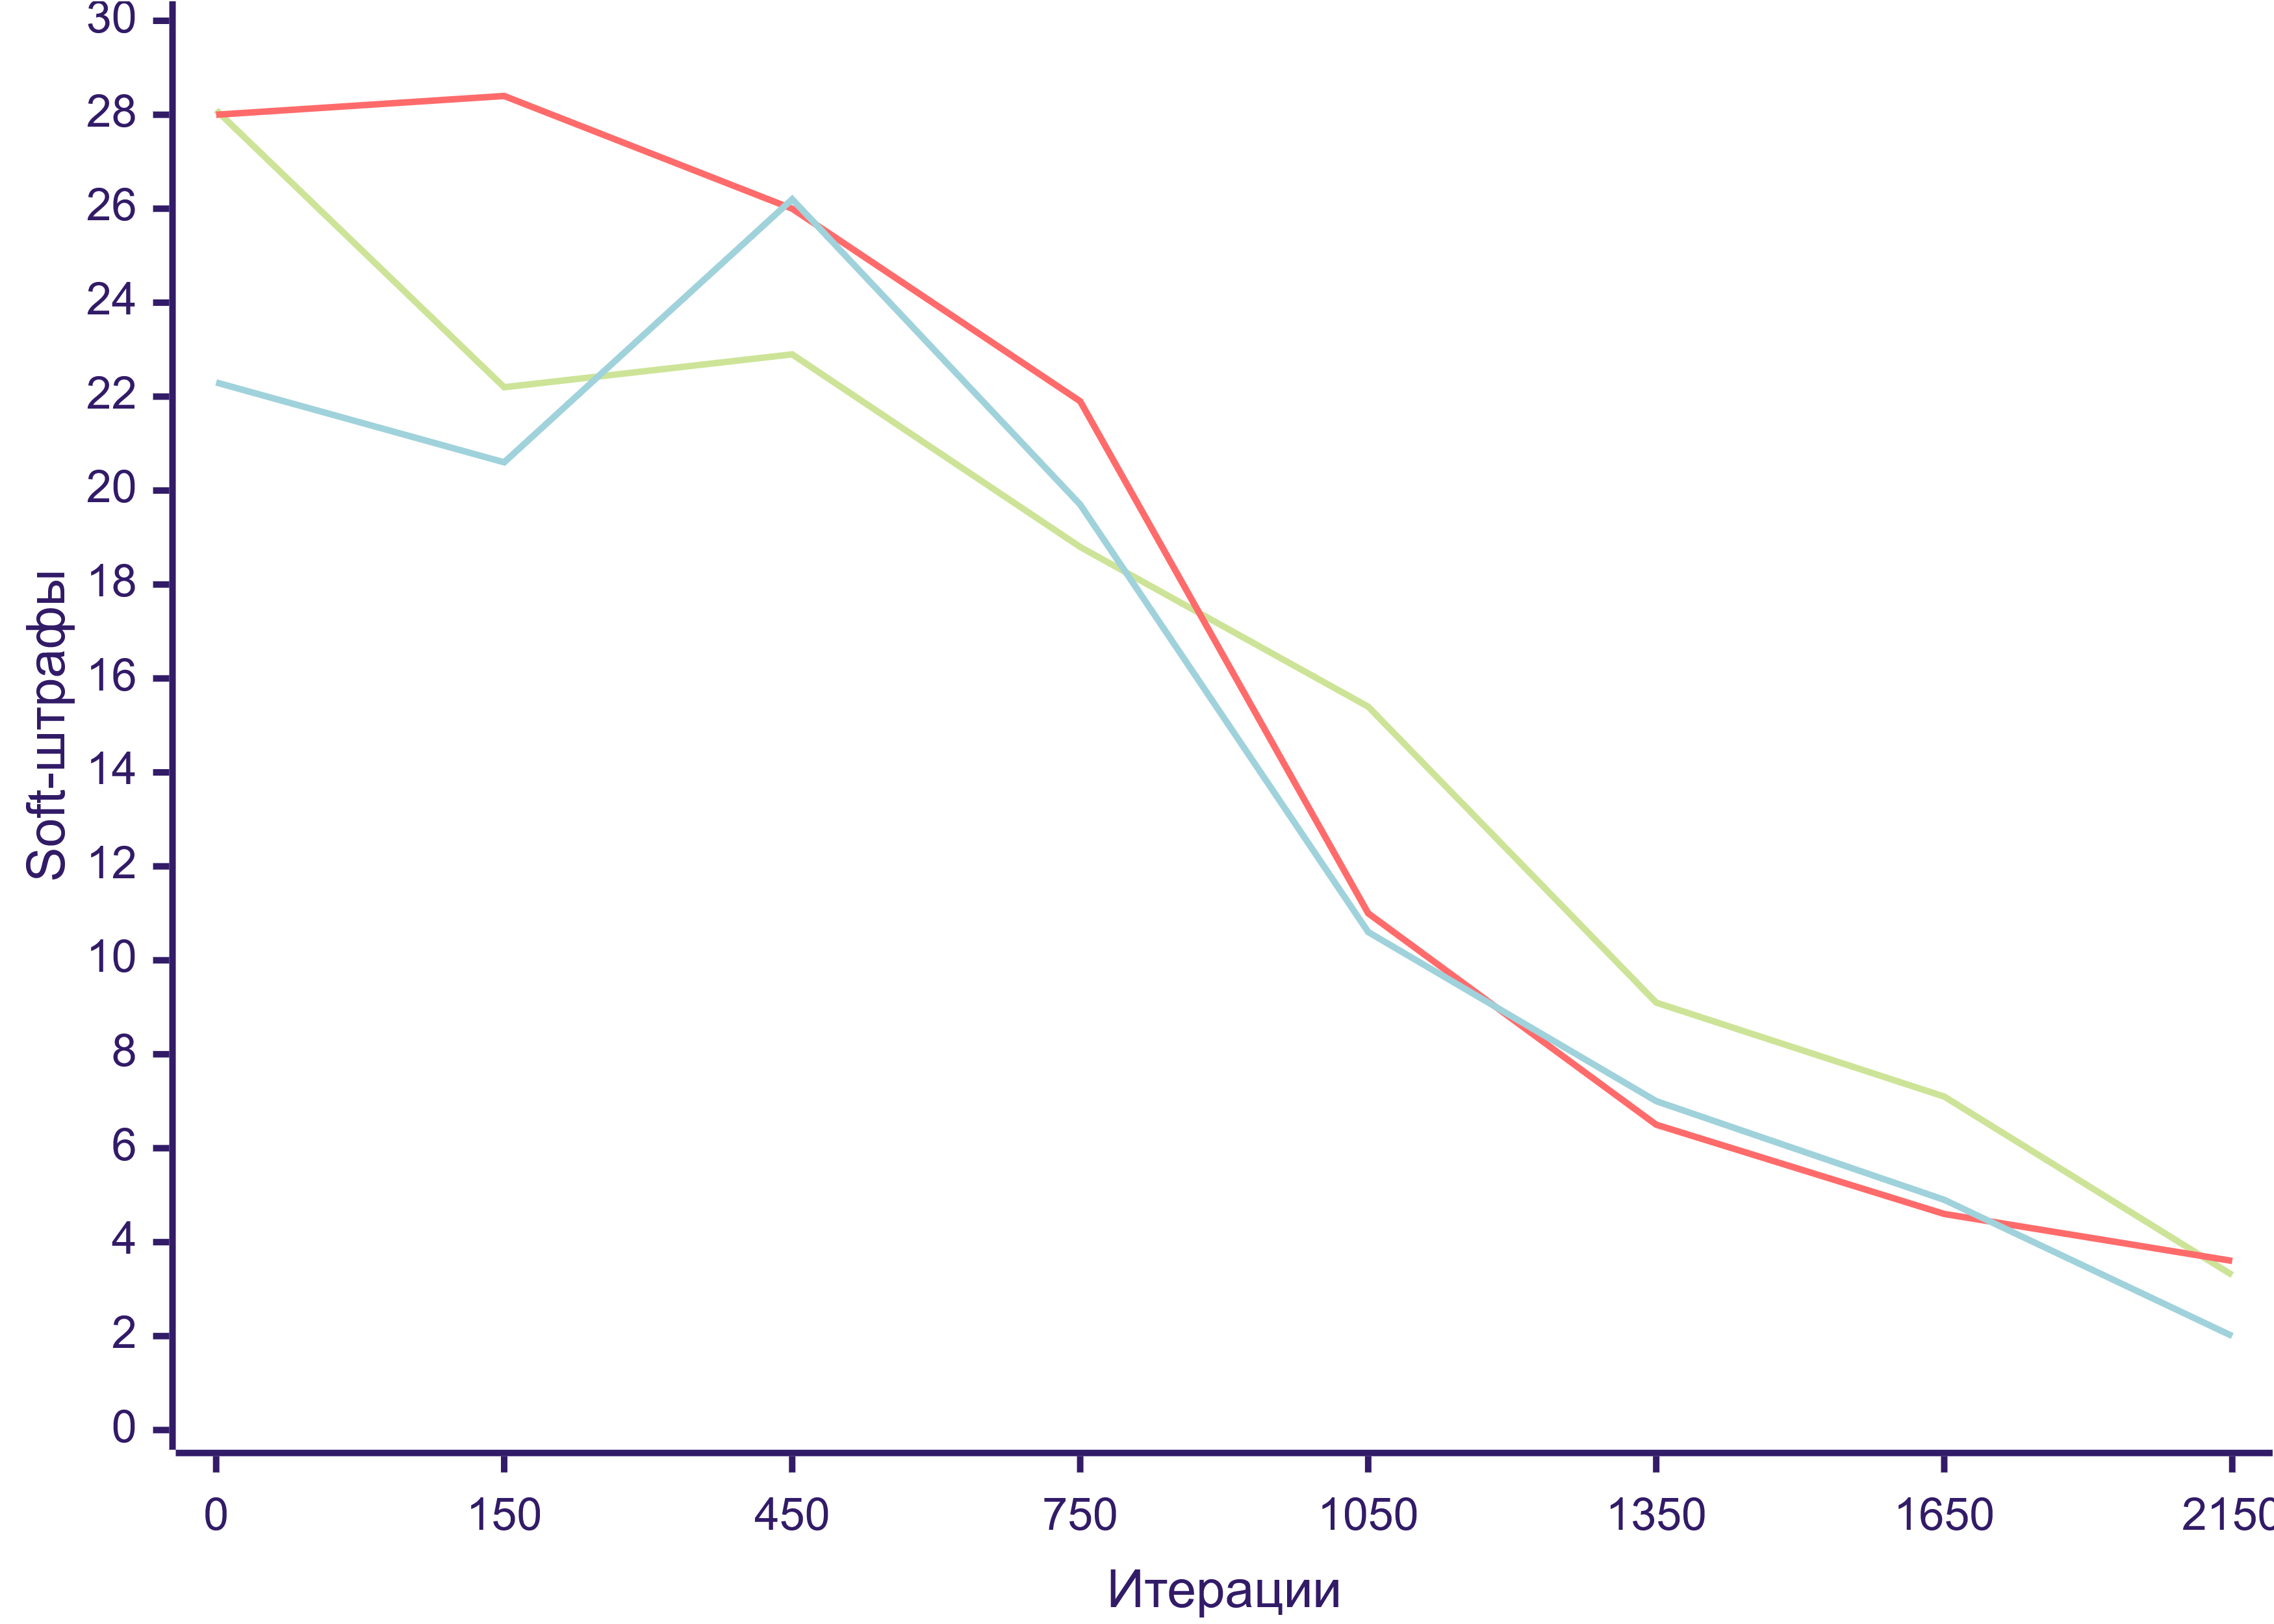
\includegraphics[width=0.8\textwidth]{images/SA Convergence.png}
    \caption{Сходимость SA: динамика soft-штрафов (medium)}
    \label{fig:SAConvergence}
\end{figure}

\paragraph {Анализ влияния гиперпараметров}

Экспериментально установлено, что эффективность метода имитации отжига критически зависит от стратегии охлаждения. При выборе высокой скорости охлаждения (cooling_rate = 0.999), мы наблюдаем прямую зависимость итогового качества решения от начальной температуры (initial_temperature). Увеличение начальной температуры до 200 позволяет алгоритму эффективнее преодолевать локальные оптимумы, обеспечивая снижение среднего штрафа с 0.95 до 0.84.

\begin{figure}[h]
    \centering
    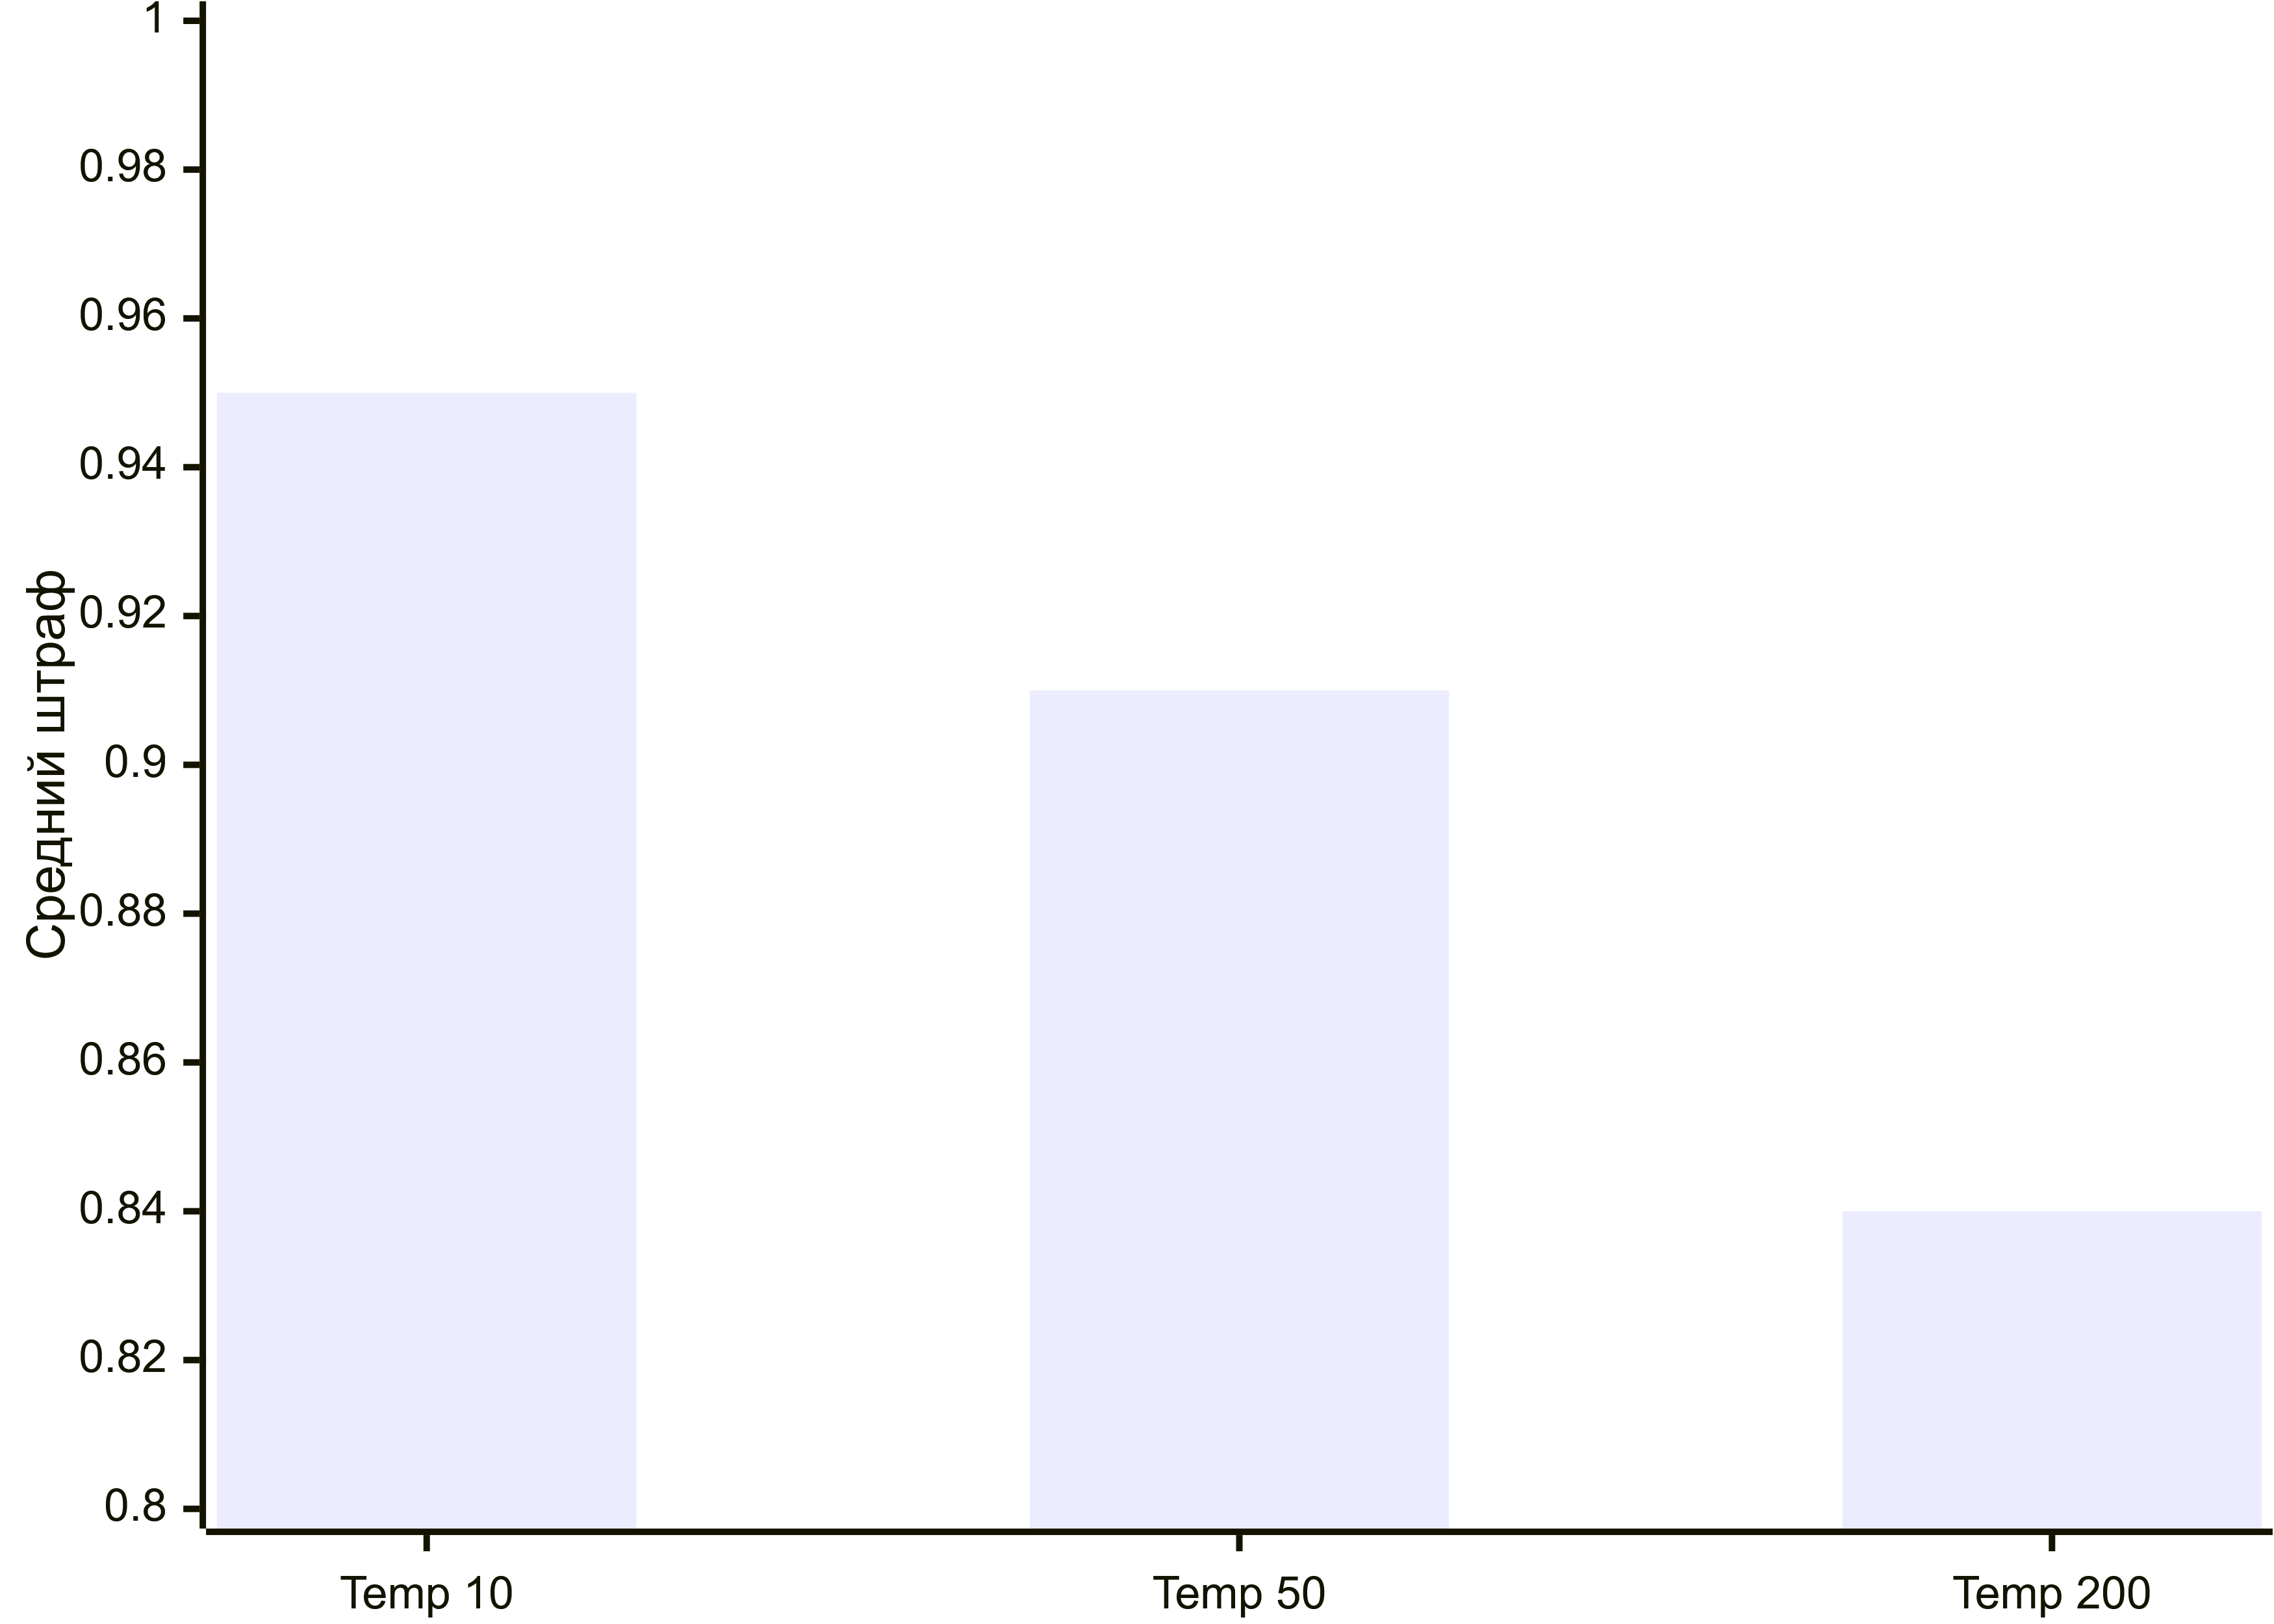
\includegraphics[width=0.8\textwidth]{images/SA Temperature.png}
    \caption{Зависимость штрафа от начальной температуры}
    \label{fig:SAtemperature}
\end{figure}

\subsubsection{ Проблемы, возникшие в процессе реализации}

В процессе анализа выбранных по умолчанию числовых параметров алгоритма была выявлена содержательная, хотя и не приводящая к видимому сбою, проблема масштаба. Коэффициент, с которым число нарушений жёстких ограничений входит в сводное числовое значение энергии, выбран заведомо большим по отношению к типичным значениям штрафа по мягким критериям — это сделано намеренно, чтобы любое ухудшение по жёстким ограничениям всегда расценивалось как существенно более плохое решение, чем любое ухудшение по мягким. Однако стартовое значение температуры было выбрано без учёта этого масштаба и оказалось на порядки меньше, чем типичная разница энергий при изменении числа жёстких нарушений на единицу. Это привело к тому, что вероятность принять ход, временно увеличивающий число жёстких нарушений ради последующего выхода из локального оптимума — то есть к самой сути метода имитации отжига, — оказывается на практике пренебрежимо малой: алгоритм фактически ведёт себя как обычный жадный локальный поиск по отношению к жёстким ограничениям, и только по отношению к мягким критериям действительно «отжигается» так, как это задумано методом. Эта проблема не была обнаружена через сбой или ошибку в логах, а была выявлена аналитически, при сопоставлении порядков величин двух связанных, но независимо выбранных числовых параметров — что говорит о необходимости содержательной, а не только эмпирической проверки гиперпараметров эвристических алгоритмов перед их использованием в сравнительном эксперименте.

Кроме того, имитация отжига в данной работе разделяла с генетическим алгоритмом и поиском с запретами общий дефект, связанный с ограничением на максимальный размер итогового расписания: контейнер для финального результата создавался с ограничением, равным вместимости учебной сетки, а не числу занятий в задаче, что на крупном наборе данных приводило к незаметному усечению расписания и, как следствие, к ложно оптимистичной оценке его допустимости. Дефект был обнаружен и устранён одинаковым образом во всех трёх затронутых реализациях.

\subsubsection{ Выводы по алгоритму}

Имитация отжига оказалась самым быстрым из четырёх реализованных алгоритмов при стабильно приемлемом качестве решения, уступающем поиску с запретами, но превосходящем генетический алгоритм. Это согласуется с тем, что метод работает с одним решением и одним недорогим по сравнению с популяционным подходом ходом за итерацию, при этом не тратя время на поддержание и пересчёт памяти о предыдущих состояниях, как это делает поиск с запретами. Вместе с тем выявленная проблема масштаба между коэффициентом штрафа за жёсткие нарушения и стартовой температурой показывает, что качество работы имитации отжига существенно зависит от тщательного согласования числовых параметров между собой, а не только от их отдельного разумного выбора.

\subsection{Поиск с запретами (Tabu Search)}
 
\subsubsection { Общие принципы и введение в алгоритм}

Поиск с запретами, как и имитация отжига, относится к методам локального поиска: алгоритм удерживает одно текущее решение и на каждом шаге пытается перейти к соседнему решению, отличающемуся от текущего одним небольшим изменением. Принципиальное отличие от имитации отжига — в способе борьбы с локальными оптимумами. Вместо вероятностного принятия ухудшающих ходов поиск с запретами ведёт явную кратковременную память о недавно совершённых изменениях и временно запрещает (заносит в табу-список) возврат к тем состояниям, из которых алгоритм только что вышел. Это позволяет алгоритму намеренно выбирать на каждом шаге наилучший из доступных соседних вариантов, даже если он хуже текущего решения — то есть осознанно двигаться «в гору» по критерию качества, не рискуя при этом немедленно вернуться назад и зациклиться между двумя соседними состояниями. Единственное исключение из запрета — критерий устремления (aspiration criterion): если запрещённый ход всё равно ведёт к лучшему решению, чем самое лучшее из найденных за всё время работы алгоритма, запрет на этот ход снимается, поскольку явная польза от такого хода перевешивает риск зацикливания.
 
Готовая, в данном случае публичная реализация поиска с запретами (репозиторий edgarsmdn/TS, тот же, что первоначально рассматривался для имитации отжига) была отклонена по той же причине, что и dual_annealing: она реализует поиск с запретами для непрерывных задач, где соседство задаётся через сужающийся радиус вокруг текущей точки в пространстве вещественных чисел, а табу-зона — это область вокруг недавно посещённых точек в этом непрерывном пространстве. У задачи расписания нет естественной метрики «расстояния» между двумя расписаниями, а ход — это не «шаг в случайном направлении», а конкретное, дискретное изменение одного занятия. Поэтому был реализован классический комбинаторный вариант поиска с запретами, восходящий к работам Фреда Гловера, с табу-списком, основанным не на расстоянии между решениями, а на запрете повторения конкретных атрибутов изменения.

\subsubsection { Особенности реализации}

На каждой итерации алгоритм генерирует не один, а целый пакет случайных ходов-кандидатов (типичный размер пакета — около двадцати пяти ходов четырёх видов: изменение дня и пары занятия, замена аудитории, замена преподавателя, обмен временными слотами между двумя занятиями) и выбирает среди них наилучший допустимый — допустимый в смысле «не запрещённый табу-списком либо проходящий по критерию устремления». Если весь пакет кандидатов оказался под запретом, выбирается случайный ход без какой-либо дополнительной проверки — это единственный встроенный механизм диверсификации поиска при затяжном застое.

Табу-список устроен не как список запрещённых полных решений (что было бы естественно для непрерывной версии алгоритма, но бессмысленно для дискретной задачи — вероятность повторно попасть ровно в то же самое расписание из миллионов возможных пренебрежимо мала), а как список запрещённых атрибутов изменения: запоминается не «то самое прошлое расписание», а конкретная связка «дисциплина — вид изменения — прежнее значение», и в течение заданного числа итераций запрещается возвращать именно эту дисциплину именно к этому прежнему значению.

\captionof{listing}{Пример запрета: запрет предыдущего слота}
\begin{minted}{python}
tabu_attrs = [(discipline_id, "slot", (old_weekday, old_timeslot))]
\end{minted}

\subsubsection { Метрики}

\paragraph { Оптимизация размера окрестности поиска}

Мы проанализировали влияние размера батча кандидатов на качество и скорость работы алгоритма. Было выявлено, что увеличение параметра neighborhood_size до 50 не приводит к дальнейшему снижению штрафов, создавая избыточную вычислительную нагрузку. Оптимальным компромиссом для рассматриваемых размерностей является значение 25.

\begin{figure}[h]
    \centering
    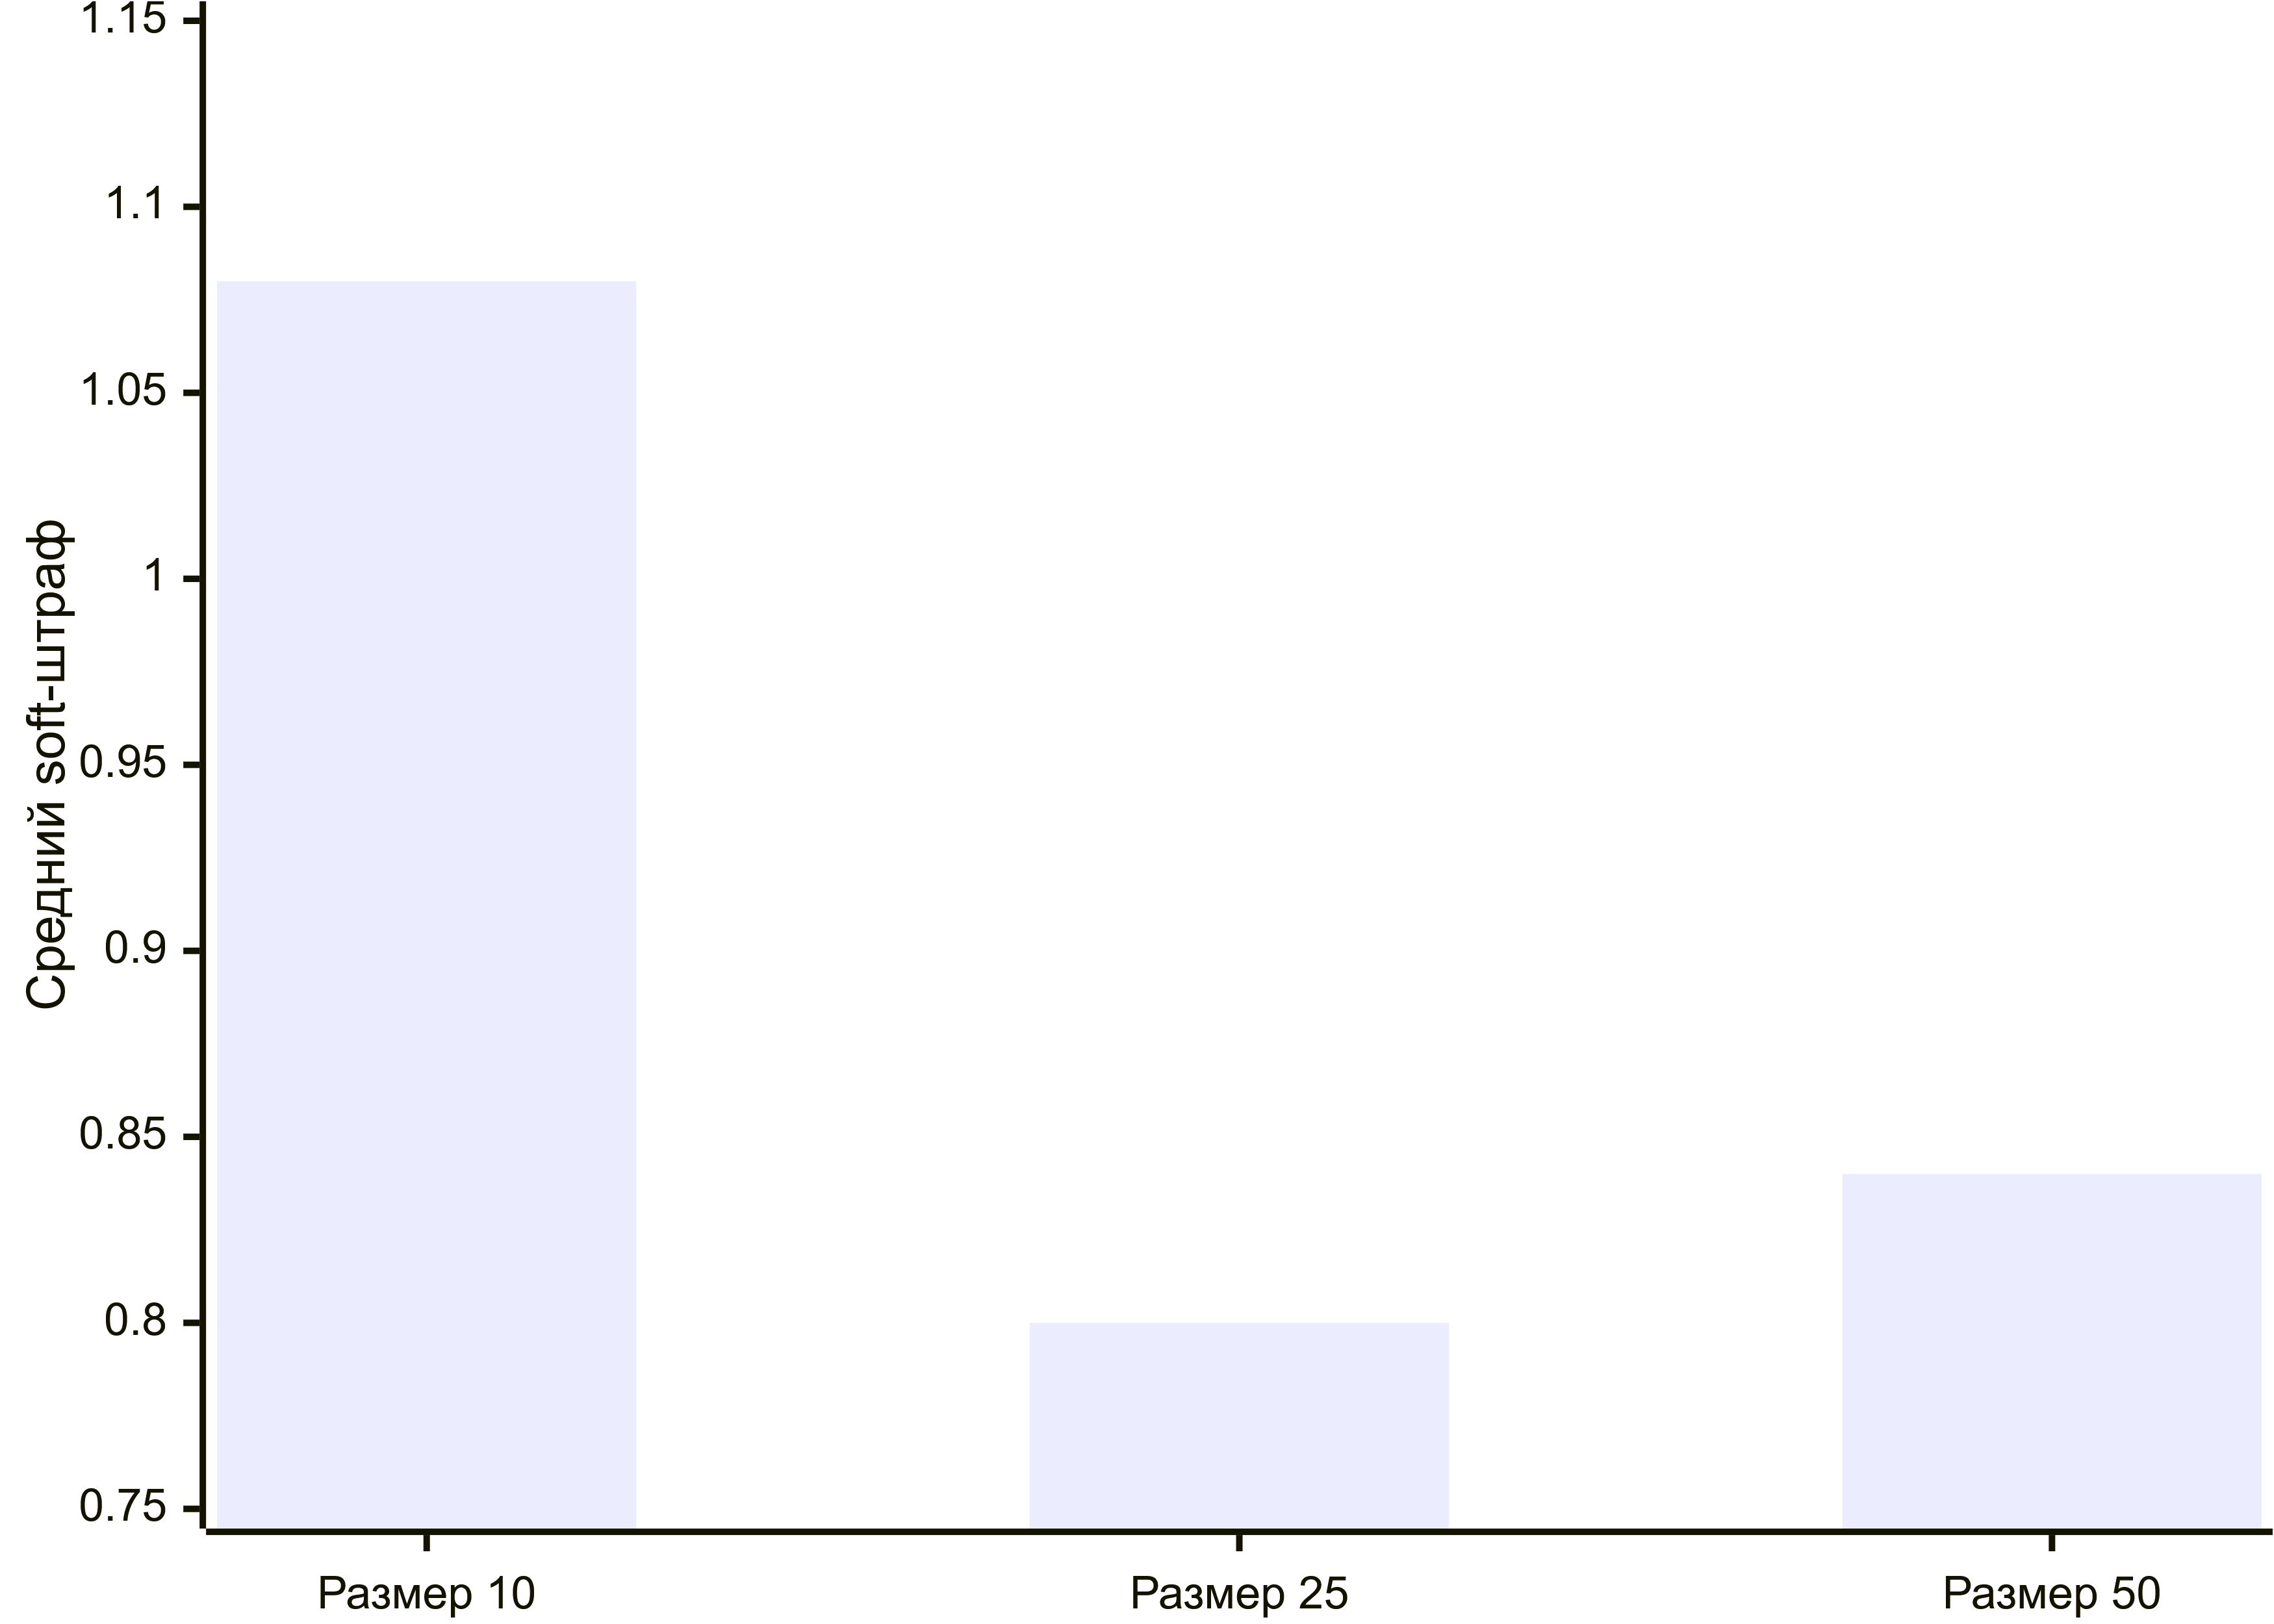
\includegraphics[width=0.8\textwidth]{images/TS neighborhood diff.png}
    \caption{Влияние neighborhood_size на качество решения}
    \label{fig:TSNeighborhoodDiff}
\end{figure}

\paragraph { Динамика поиска}

Процесс сходимости TS носит ступенчатый характер. Выбор лучшего кандидата из окрестности на каждой итерации обеспечивает резкие улучшения целевой функции, которые сменяются периодами стагнации (плато) при достижении локального минимума в рамках текущего региона поиска.

\begin{figure}[h]
    \centering
    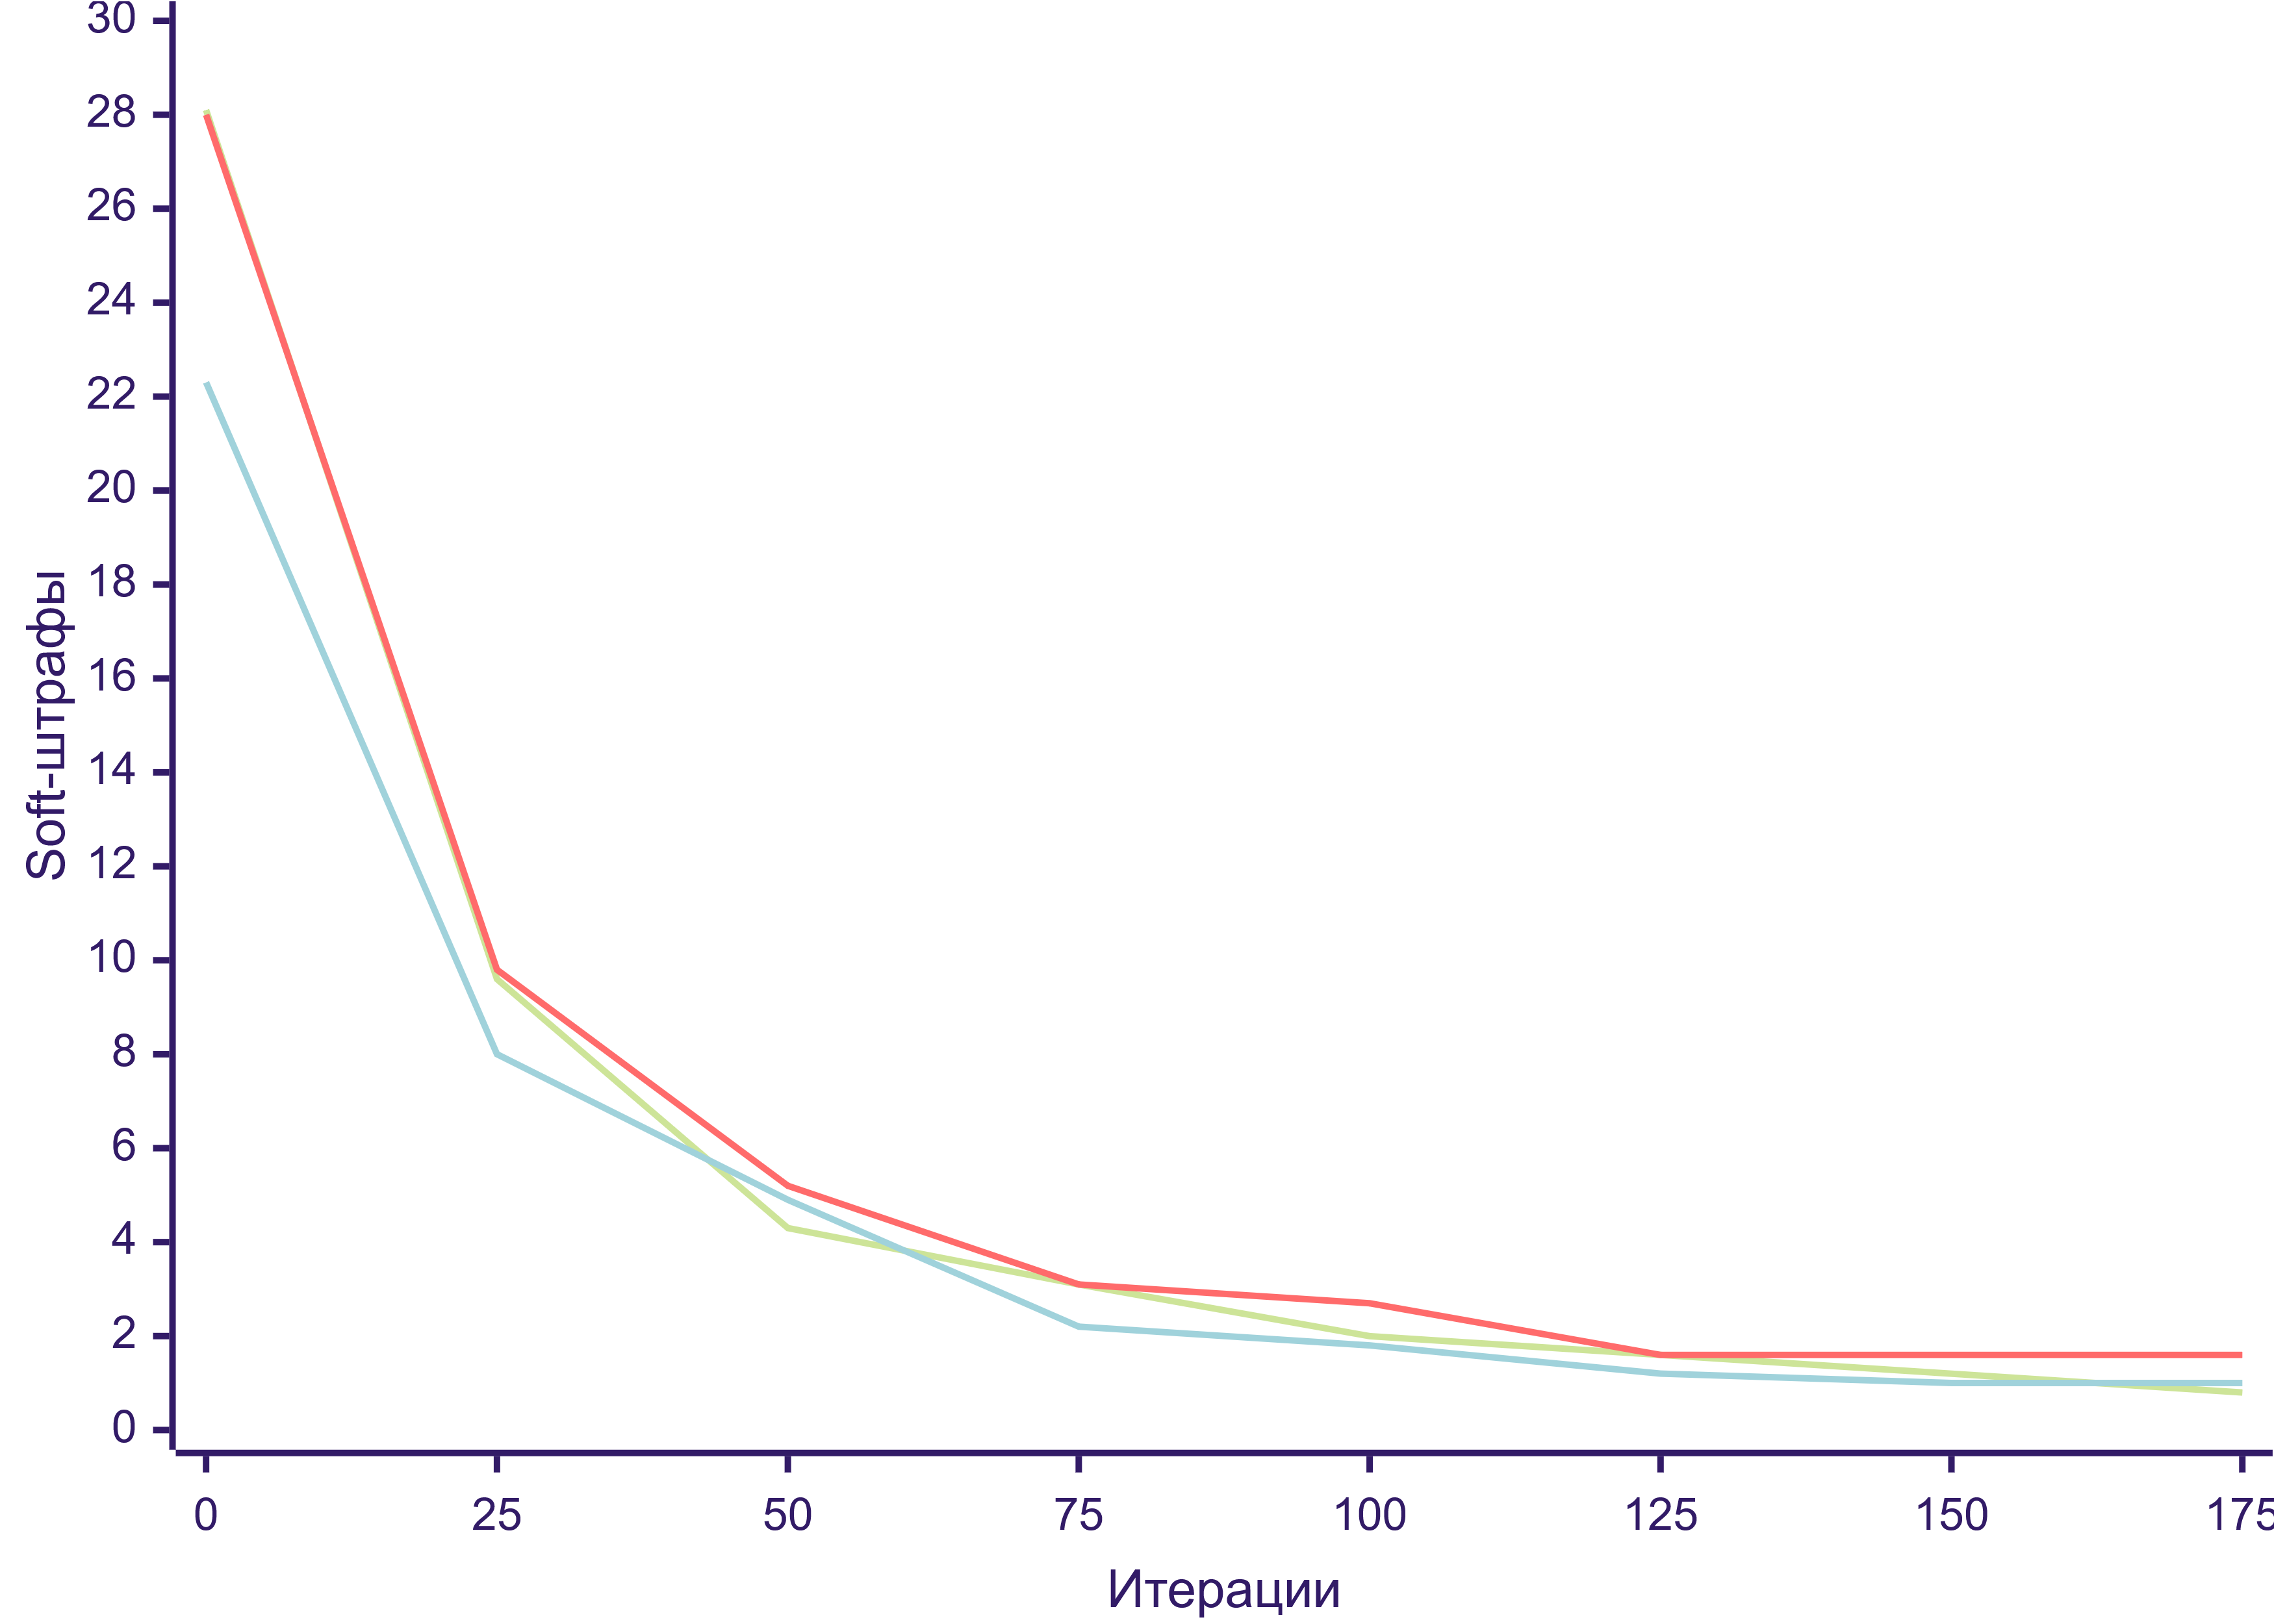
\includegraphics[width=0.8\textwidth]{images/TS Convergence.png}
    \caption{Сходимость TS: динамика soft-штрафов (medium)}
    \label{fig:TSConvergence}
\end{figure}

\subsubsection { Проблемы, возникшие в процессе реализации}

При сопоставлении поиска с запретами с точным методом программирования ограничений (раздел II.4) на крупном наборе данных, заведомо превышающем физическую вместимость учебной сетки, был обнаружен дефект, общий с генетическим алгоритмом и имитацией отжига: контейнер для итогового расписания создавался с ограничением на число занятий, равным вместимости учебной сетки, а не реальному числу занятий в задаче, и лишние занятия незаметно отбрасывались при сборке результата. Особенно показательно, что именно точный метод программирования ограничений — за счёт способности доказывать отсутствие допустимого решения, а не просто сообщать о неудаче поиска — стал той самой опорной точкой, которая позволила опровергнуть ложный вывод о допустимости расписания, построенного поиском с запретами: при заведомой невозможности уместить все занятия в доступные пары точный метод сообщал об отсутствии решения, тогда как поиск с запретами сообщал о найденном допустимом расписании без единого нарушения, что было логическим противоречием, потребовавшим целевой диагностики и приведшим к обнаружению описанного дефекта.

Отдельная архитектурная особенность, выявленная при анализе кода, но не успевшая проявиться в виде наблюдаемой ошибки в рамках проведённого эксперимента, — это потенциальная неоднозначность атрибута табу-запрета в ситуации, когда у одной дисциплины несколько занятий в неделю (например, две лекции). Поскольку запрет привязывается к идентификатору дисциплины, а не к конкретному занятию, теоретически возможна ситуация, при которой запрет, наложенный из-за хода с одним занятием этой дисциплины, ошибочно распространится на другое занятие той же дисциплины, никогда не находившееся в запрещённом состоянии. Это не привело к видимому снижению качества решений в проведённом эксперименте, но обозначено как направление для дальнейшего уточнения реализации.

\subsubsection { Выводы по алгоритму}

Поиск с запретами стабильно показал наилучшее качество решений среди всех четырёх реализованных алгоритмов на всех использованных наборах данных, включая случай, когда задача оказалась структурно неразрешимой и сравнение шло по числу остаточных, неустранимых нарушений. По затраченному времени поиск с запретами оказался медленнее имитации отжига, что объясняется оценкой целого пакета кандидатов на каждой итерации вместо одного хода, но при этом существенно быстрее генетического алгоритма. Сочетание лучшего качества решения с умеренными вычислительными затратами делает поиск с запретами наиболее сбалансированным из четырёх реализованных эвристических методов для рассматриваемой задачи.

\subsection{Программирование ограничений (Constraint Programming / CP-SAT)}
 
\subsubsection { Общие принципы и введение в алгоритм}

Программирование ограничений — это принципиально иной подход к задаче по сравнению с тремя рассмотренными ранее. Генетический алгоритм, имитация отжига и поиск с запретами — это метаэвристики: они исследуют пространство решений, проверяя сами решения на допустимость постфактум, и не гарантируют ни нахождения наилучшего решения, ни даже корректного определения того, что решения вовсе не существует. Решатель ограничений работает иначе: вместо того чтобы перебирать готовые решения и штрафовать их за нарушения, он описывает задачу как набор переменных с ограниченными областями допустимых значений и набор логических связей между ними, а затем находит значения всех переменных, удовлетворяющие всем связям одновременно, либо строго доказывает, что таких значений не существует. Использованный в данной работе решатель CP-SAT (Constraint Programming — Satisfiability) из состава библиотеки Google OR-Tools объединяет в себе классический аппарат программирования ограничений с современными методами решения задач булевой выполнимости (SAT), что делает его одним из самых быстрых открытых решателей такого класса задач на сегодняшний день.

Принципиальное практическое следствие этого различия — то, как в решателе ограничений реализуются жёсткие ограничения. В трёх предыдущих алгоритмах жёсткое ограничение — это функция, которая после построения кандидата решения проверяет, не нарушено ли оно, и в случае нарушения штрафует решение численно. В CP-SAT жёсткое ограничение, где это возможно, реализуется не как проверка постфактум, а как сужение области допустимых значений переменной заранее: например, переменная «преподаватель данного занятия» с самого начала может принимать только те значения, которые соответствуют преподавателям, действительно квалифицированным по данной дисциплине, — недопустимое значение просто не существует как вариант, и проверять его на допустимость после не требуется.

\subsubsection { Особенности реализации}

Каждое занятие, которое требуется расставить, описывается набором переменных: день недели, номер пары, индекс аудитории внутри заранее отфильтрованного по вместимости и типу списка подходящих аудиторий, и аналогично — индекс преподавателя внутри списка квалифицированных по дисциплине преподавателей. Использование индекса внутри уже отфильтрованного списка, а не прямого идентификатора аудитории или преподавателя, — это и есть тот самый механизм сужения области допустимых значений: недопустимые комбинации физически не входят в эти списки, и решателю не нужно объяснять отдельным правилом, что аудитория должна вмещать группу или что преподаватель должен быть квалифицирован.

Уникальность временного слота занятия — единственное жёсткое ограничение, требующее отдельной явной формулировки, поскольку оно связывает между собой все занятия сразу, а не одно занятие с его собственными параметрами. Для этого день и номер пары каждого занятия объединяются в единый числовой код слота, и накладывается ограничение на то, что все такие коды должны быть попарно различны.

\captionof{listing}{Обьявление всех слотов для предотвращения конфликтов}
\begin{minted}{python}
model.add_all_different([v.slot_id for v in session_vars])
\end{minted}

Любопытное наблюдение, сделанное в процессе формализации модели: ограничение на максимально допустимое число занятий в один день, которое в остальных трёх алгоритмах реализовано отдельной проверяющей функцией, в формулировке через решатель ограничений оказывается автоматическим следствием уже описанного ограничения на уникальность слота в сочетании с тем, что номер пары и так ограничен сверху вместимостью учебного дня: если бы в один день нужно было поставить больше занятий, чем число доступных номеров пар, какие-то два занятия неизбежно получили бы одинаковый номер пары, что само по себе уже запрещено ограничением уникальности. Это пример того, как формальная постановка задачи в виде ограничений иногда вскрывает логические связи между условиями, которые при процедурной, проверочной реализации остаются незамеченными и формулируются как будто бы независимо друг от друга.

Поскольку решатель ограничений требует, чтобы итоговая минимизируемая величина была линейной функцией переменных, один из мягких критериев качества — равномерность загрузки по дням недели, которая в остальных трёх алгоритмах выражена через дисперсию числа занятий по дням, — была заменена на линейный аналог: разницу между максимальной и минимальной загрузкой дня. Это сохраняет содержательный смысл критерия — штраф за неравномерность — но не совпадает с дисперсией число в число, что является осознанным и явно задокументированным отступлением от полной идентичности критериев качества между всеми четырьмя алгоритмами.

\subsubsection { Метрики}

\paragraph{ Стабильность решения при изменении временного бюджета}

Результаты прогонов подтверждают высокую эффективность CP-SAT для размерностей типа medium. Алгоритм доказывает глобальную оптимальность решения в рамках первых 200–210 мс, что делает избыточным выделение значительного временного бюджета.

*Рисунок II.3. Фактическое время работы солвера при различных временных ограничениях*

\begin{figure}[h]
    \centering
    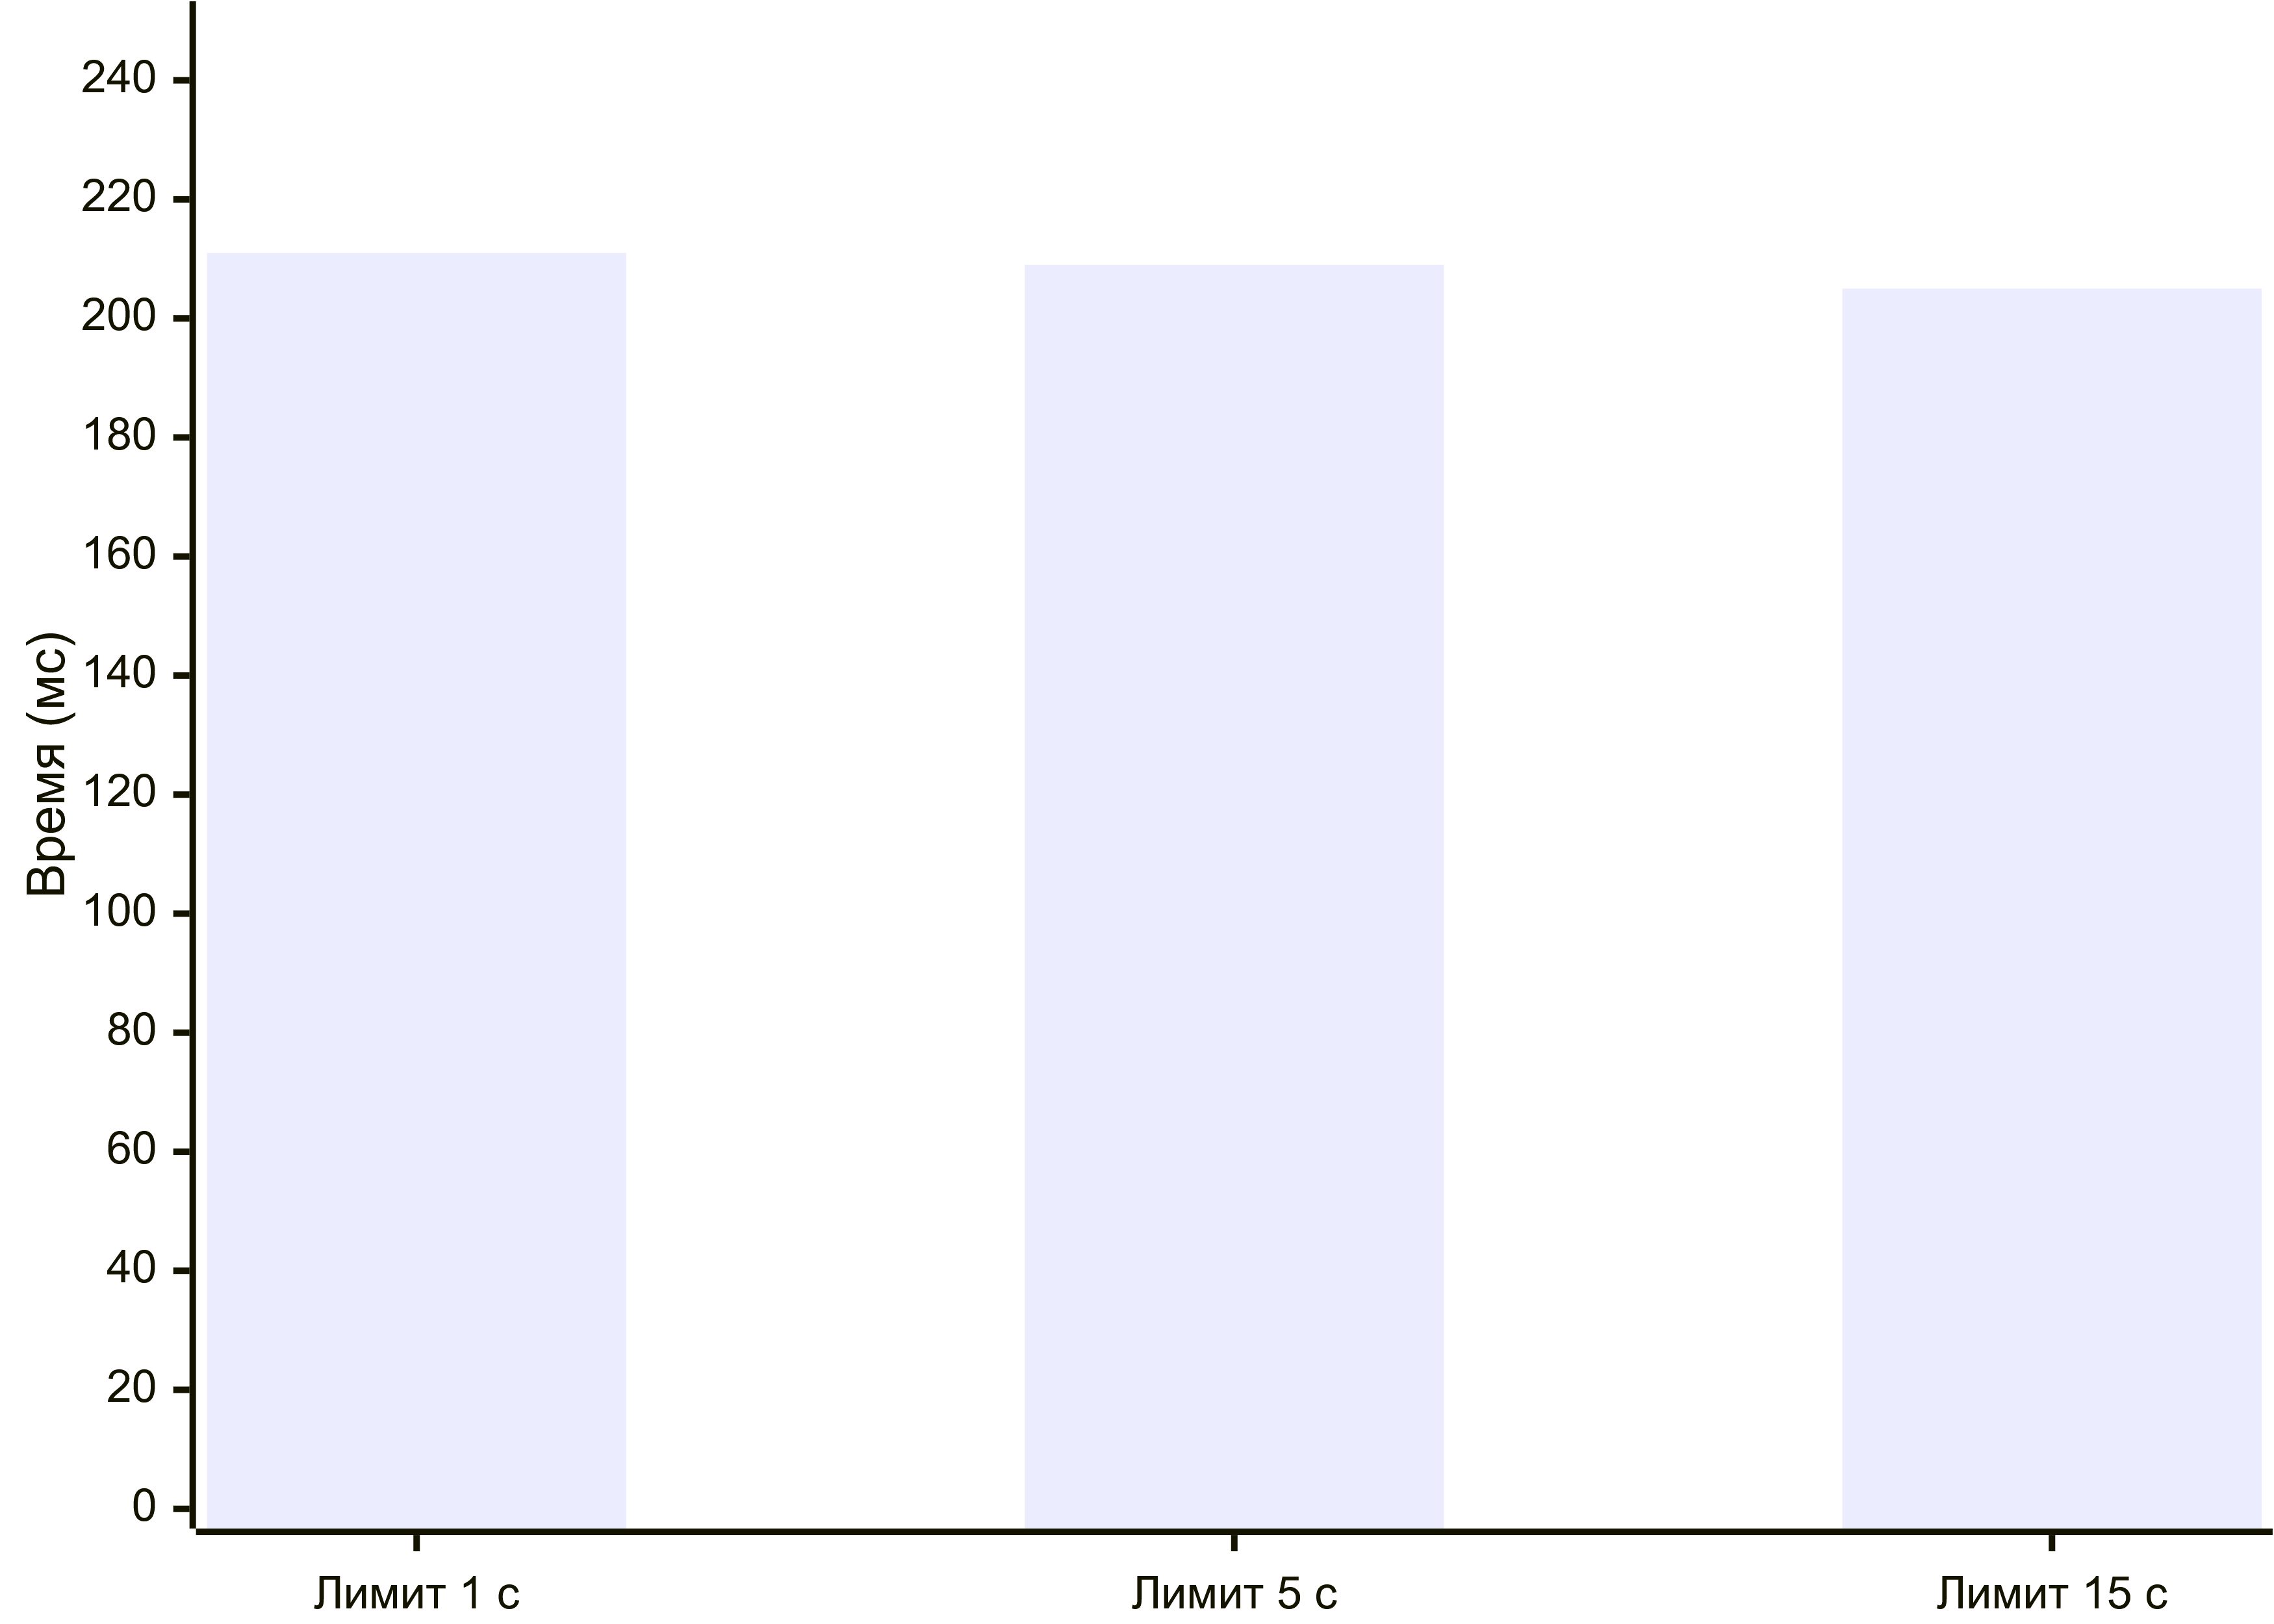
\includegraphics[width=0.8\textwidth]{images/CP Extra Time.png}
    \caption{Фактическое время вычислений при изменении бюджета}
    \label{fig:CPExtraTime}
\end{figure}

\subsubsection { Проблемы, возникшие в процессе реализации}

Основная сложность при формализации модели была связана с вычислением показателя компактности занятий в течение дня — числа «окон» между первым и последним занятием дня. В отличие от трёх остальных алгоритмов, где это вычисляется прямым проходом по уже готовому, полностью определённому расписанию, в решателе ограничений на момент формулировки модели неизвестно, какие именно занятия попадут на какой день — это сама переменная, которую решатель должен подобрать. Потребовалось ввести вспомогательные логические переменные-индикаторы «это занятие стоит в этот день» и связать с их помощью минимальный и максимальный номер пары среди занятий каждого дня, отдельно обработав вырожденный случай дня без единого занятия — без этой отдельной обработки решатель мог бы произвольно манипулировать значениями вспомогательных переменных на пустых днях, искусственно занижая итоговый штраф без какой-либо связи с реальным расписанием.

Корректность итоговой формулировки была дополнительно подтверждена тем, что после нахождения решения оно прогонялось через тот же самый, общий для всех четырёх алгоритмов расчёт количества нарушений жёстких и мягких ограничений: расчёт во всех случаях подтверждал нулевое число жёстких нарушений, что и должно было быть гарантировано самой природой решателя ограничений, а не результатом случайного совпадения.

\subsubsection { Выводы по алгоритму}

Решатель ограничений на всех наборах данных, где допустимое решение существовало, находил решение, доказанно не худшее, чем найденное любым из трёх эвристических алгоритмов, и в большинстве случаев находил его за сопоставимое или меньшее время. На наборе данных, где допустимого решения не существовало вовсе из-за структурного несоответствия между числом занятий и вместимостью учебной сетки, решатель ограничений единственный из всех четырёх алгоритмов дал не просто отрицательный, а доказанный ответ — притом за время, существенно меньшее, чем у любого из эвристических методов, поскольку для доказательства отсутствия решения решателю не требуется производить полноценный поиск по всему пространству вариантов. Это свойство — способность не просто не найти решение, а строго доказать его отсутствие, — оказалось практически значимым и за пределами чисто академического интереса: именно противоречие между ответом решателя ограничений и ответами трёх эвристических алгоритмов на одном и том же наборе данных послужило прямым указанием на дефект реализации, описанный в разделах II.1–II.3.

\subsection{Сравнительный анализ алгоритмов)}
 
\subsubsection { Методика сравнения}

Сравнение четырёх алгоритмов строилось на единой модели данных и едином критерии оценки качества решения — паре чисел «количество нарушенных жёстких ограничений, суммарный штраф по мягким ограничениям», вычисляемой одной и той же функцией независимо от того, какой алгоритм построил расписание. Без этого условия сравнение было бы лишено смысла: разные единицы измерения качества у разных алгоритмов сделали бы любые числовые выводы недостоверными.

Сравнение проводилось по двум независимым осям, которые отвечают на разные вопросы и не должны подменять друг друга. Первая ось — повторные запуски одного и того же алгоритма на одном и том же наборе данных с разными случайными начальными значениями (от одного до десяти запусков на комбинацию алгоритма и набора данных). Эта ось отвечает на вопрос об устойчивости результата: насколько сильно качество решения, найденного генетическим алгоритмом, имитацией отжига или поиском с запретами, зависит от случайности, заложенной в эти методы. Вторая ось — использование нескольких наборов исходных данных разного размера и разной степени структурной сложности. Эта ось отвечает на принципиально другой вопрос: насколько обнаруженные закономерности обобщаются за пределы одного конкретного набора данных. Подмена одной оси другой — типичная методическая ошибка при сравнении эвристических алгоритмов: устойчивый результат на единственном наборе данных ничего не говорит о том, как алгоритм поведёт себя на задаче другого размера.

Дополнительно как точка опоры использовался метод полного перебора с откатом — переборный алгоритм, не входящий в основной список сравниваемых методов, но применённый для подтверждения корректности остальных реализаций на заведомо малых, заранее проверяемых вручную фрагментах задачи. Поскольку полный перебор для задачи такого размера, как использованные в основном эксперименте наборы данных, физически неосуществим за разумное время, его роль ограничена ролью независимого арбитра на крошечных тестовых случаях, а не участника основного сравнения.

\subsubsection { Наборы данных}

Для эксперимента были подготовлены четыре синтетических набора данных программным генератором, не зависящим от системы управления базами данных, что позволило точно контролировать как размер задачи (число дисциплин, аудиторий, преподавателей), так и её структурную сложность (число преподавателей, квалифицированных по каждой дисциплине, и число типов аудиторий, подходящих под каждую дисциплину) независимо друг от друга.
\begin{table}[h]
    \centering
    \caption{Используемые наборы данных}
    \label{tab:datasets}

    \begin{tabular}{|l|c|p{4cm}|p{5cm}|}
        \hline
        \textbf{Набор данных} &
        \textbf{Занятий} &
        \textbf{Структурная сложность} &
        \textbf{Особенность} \\
        \hline

        tiny\_easy &
        9 &
        Низкая (много вариантов на каждое занятие) &
        Минимальный показательный случай \\
        \hline

        small\_tight &
        11 &
        Высокая (минимум вариантов на каждое занятие) &
        Малый размер при тугих ограничениях \\
        \hline

        medium &
        26 &
        Средняя &
        Основной показательный случай среднего масштаба \\
        \hline

        large\_stress &
        54 &
        Вместимость учебной сетки заведомо меньше числа занятий &
        Намеренно структурно неразрешимый случай \\
        \hline

    \end{tabular}
\end{table}

Набор large_stress заслуживает отдельного пояснения. Изначально он задумывался как стресс-тест на крупном, но разрешимом объёме данных, однако при заданных параметрах учебной сетки (шесть дней, семь пар в день — сорок два доступных слота) и двадцати пяти дисциплин с учётом лекционных, семинарских и лабораторных занятий суммарное число занятий, которые требовалось расставить, составило пятьдесят четыре — больше, чем физически доступных слотов. В результате этот набор данных оказался не просто «большим», а структурно неразрешимым: ни один из четырёх алгоритмов не может построить расписание без хотя бы одного нарушения жёсткого ограничения, какой бы метод и сколько бы времени ни использовалось. Решение оставить этот набор данных в эксперименте, а не исключить его как ошибочный, было принято осознанно: именно на нём наиболее наглядно проявляется разница между точным и эвристическими методами в части способности корректно распознать отсутствие решения, а не просто не найти его.

\subsubsection { Результаты на разрешимых наборах данных}

Таблица отображает используемые параметры для общих замеров.
\begin{table}[h]
    \centering
    \caption{Параметры алгоритмов и анализ гиперпараметров}
    \label{tab:hyperparameters}

    \begin{tabular}{|l|l|p{4cm}|p{5cm}|}
        \hline
        \textbf{Алгоритм} &
        \textbf{Параметр} &
        \textbf{Значение по умолчанию} &
        \textbf{Перебиралось в анализе гиперпараметров} \\
        \hline

        TS & \texttt{max\_iterations} & 500 & Нет \\
        \hline

        TS & \texttt{neighborhood\_size} & 25 & Да (10 / \textbf{25} / 50) \\
        \hline

        TS & \texttt{tabu\_tenure} & 20 & Да (10 / \textbf{20} / 40) \\
        \hline

        GA & \texttt{population\_size} & 100 & Да (50 / \textbf{100} / 200) \\
        \hline

        GA & \texttt{gene\_mut\_indpb} & 0.1 & Да (0.05 / \textbf{0.1} / 0.2) \\
        \hline

        SA & \texttt{initial\_temperature} & 50.0 & Да (10 / \textbf{50} / 200) \\
        \hline

        SA & \texttt{cooling\_rate} & 0.995 & Да (0.99 / \textbf{0.995} / 0.999) \\
        \hline

        SA & \texttt{min\_temperature} & $10^{-3}$ & Нет \\
        \hline

        SA & \texttt{max\_iterations} & 20\,000 & Нет \\
        \hline

        CP-SAT & \texttt{max\_time\_in\_seconds} & 30.0 & Нет (были 1 / 5 / 15) \\
        \hline

    \end{tabular}
\end{table}

Таблица ниже обобщает результаты на трёх наборах данных, для которых допустимое решение существует. Во всех случаях все четыре алгоритма находили решение без единого нарушения жёстких ограничений на каждом из десяти запусков; различие — в качестве решения по мягким критериям и в затраченном времени.

\begin{table}[h]
    \centering
    \caption{Сравнение алгоритмов на различных наборах данных}
    \label{tab:algorithm_comparison}

    \begin{tabularx}{\textwidth}{|l|l|c|c|c|}
        \hline
        \textbf{Набор данных} &
        \textbf{Алгоритм} &
        \textbf{Средний мягкий штраф} &
        \textbf{Отклонение от лучшего, \%} &
        \textbf{Среднее время, мс} \\
        \hline

        tiny\_easy   & CP-SAT & 0.160 & 0.0   & 51   \\
        \hline
        tiny\_easy   & TS      & 0.160 & 0.0   & 83   \\
        \hline
        tiny\_easy   & GA      & 0.160 & 0.0   & 1280 \\
        \hline
        tiny\_easy   & SA      & 0.382 & 138.9 & 53   \\
        \hline

        small\_tight & CP-SAT & 5.615 & 0.0   & 59   \\
        \hline
        small\_tight & TS      & 5.615 & 0.0   & 57   \\
        \hline
        small\_tight & GA      & 5.615 & 0.0   & 1530 \\
        \hline
        small\_tight & SA      & 5.615 & 0.0   & 58   \\
        \hline

        medium & CP-SAT & 0.799 & 0.0   & 210  \\
        \hline
        medium & TS      & 0.818 & 2.4   & 272  \\
        \hline
        medium & SA      & 2.984 & 273.4 & 92   \\
        \hline
        medium & GA      & 7.407 & 826.8 & 3210 \\
        \hline

    \end{tabularx}
\end{table}

Картина устойчиво повторяется на всех трёх наборах данных и становится тем отчётливее, чем больше размер задачи. На самом простом наборе (tiny_easy) различие между алгоритмами почти не проявляется — задача настолько слабо ограничена, что любой из методов с лёгкостью находит решение, близкое к оптимальному, кроме имитации отжига, чьё среднее значение штрафа заметно выше из-за случайных неудачных запусков (на двух из десяти запусков итоговый штраф оказался существенно выше, чем на остальных восьми, что отражает чувствительность метода к случайному стартовому состоянию на отдельных запусках). На наборе данных с тугими ограничениями (small_tight) все четыре алгоритма сошлись к одному и тому же значению на всех запусках без исключения — структура задачи здесь настолько жёстко определена малым числом допустимых комбинаций, что фактически не оставляет алгоритмам выбора. Наиболее показательный случай — набор данных среднего размера (medium), на котором различие между алгоритмами проявляется наиболее ярко: поиск с запретами почти не отстаёт от доказанно оптимального решения, найденного решателем ограничений, имитация отжига отстаёт примерно втрое, а генетический алгоритм — почти на порядок, при этом затрачивая на порядок больше времени, чем любой из трёх остальных методов.

\paragraph { Анализ производительности и устойчивости алгоритмов}

Сравнение медианных показателей времени выполнения демонстрирует существенный разрыв между математическим солвером и эвристическими методами. Генетический алгоритм требует значительно больших вычислительных ресурсов при достижении сопоставимого с TS качества.

\begin{figure}[h]
    \centering
    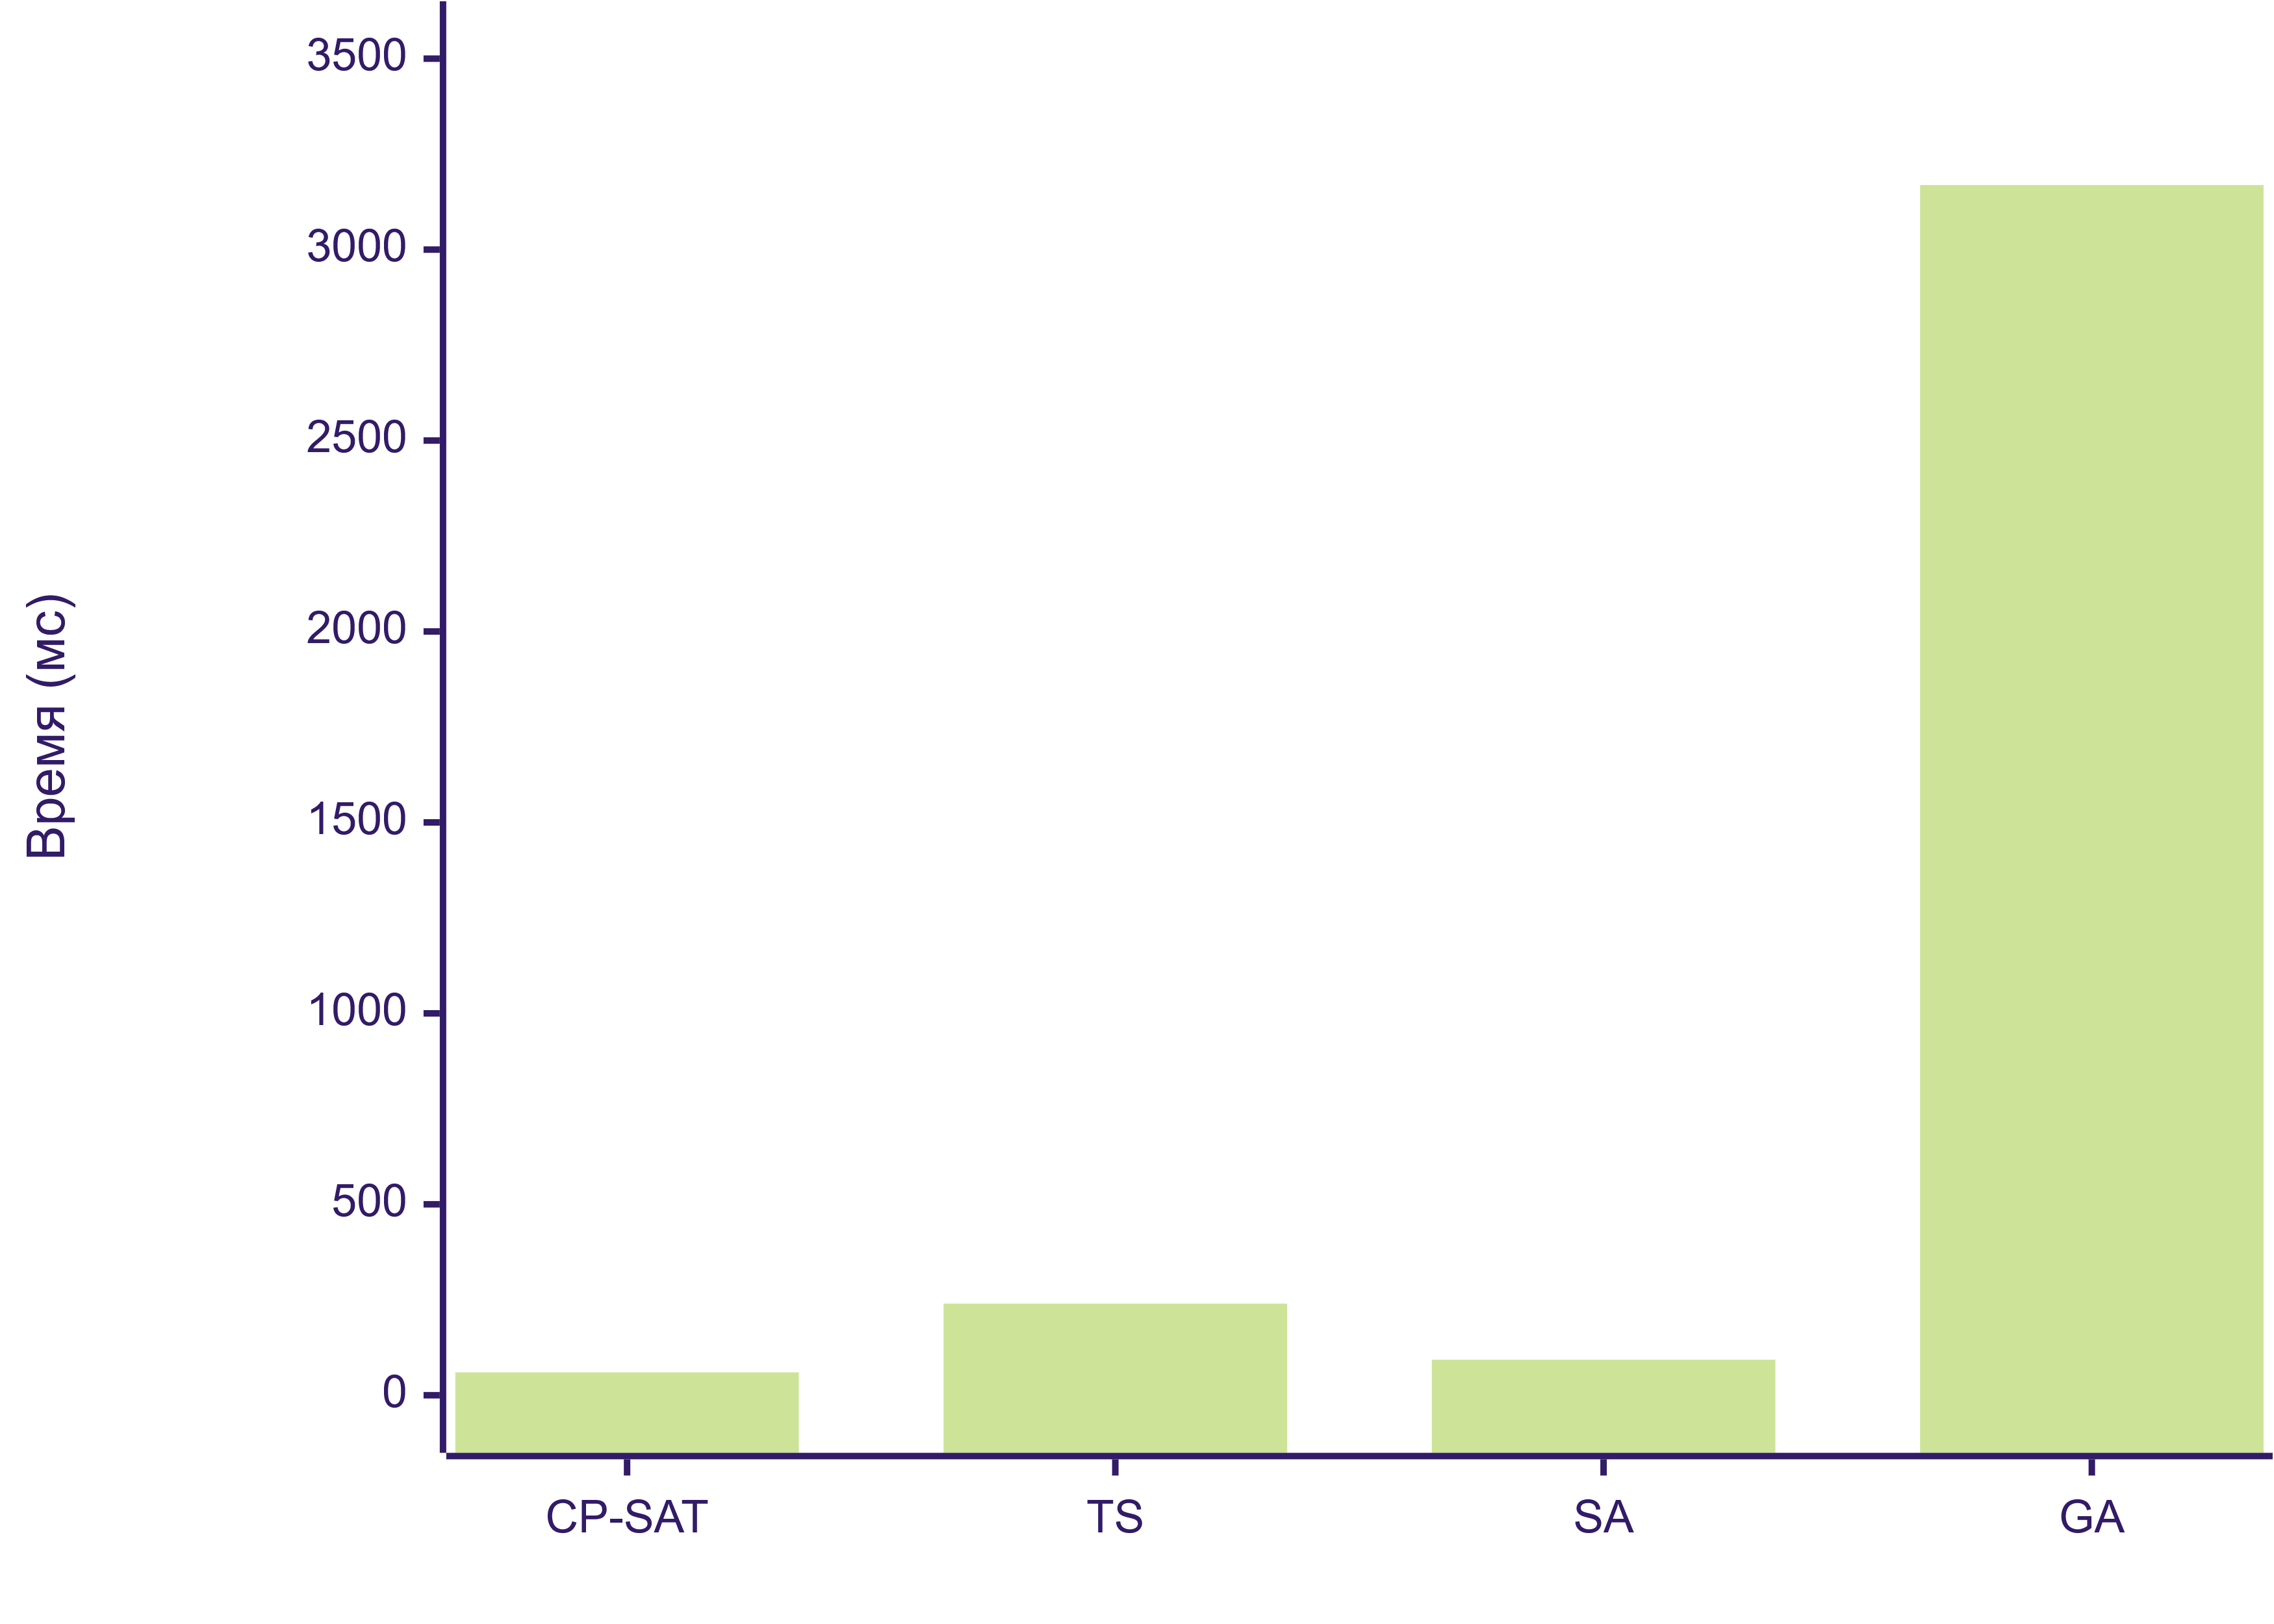
\includegraphics[width=0.8\textwidth]{images/Algorithms time diff.png}
    \caption{Сравнение медианного времени работы алгоритмов}
    \label{fig:AlgsTimeDiff}
\end{figure}

\paragraph { Эффективность эвристик в сравнении с точным методом}

Для оценки качества алгоритмов мы использовали метрику «отставания от лучшего решения» (Gap to Best). Эксперименты на датасете small_tight показали, что все рассматриваемые методы достигают глобального оптимума (0% отставания). Напротив, при усложнении задачи (датасет medium) методы начинают демонстрировать значительную дифференциацию результатов.


\begin{figure}[h]
    \centering
    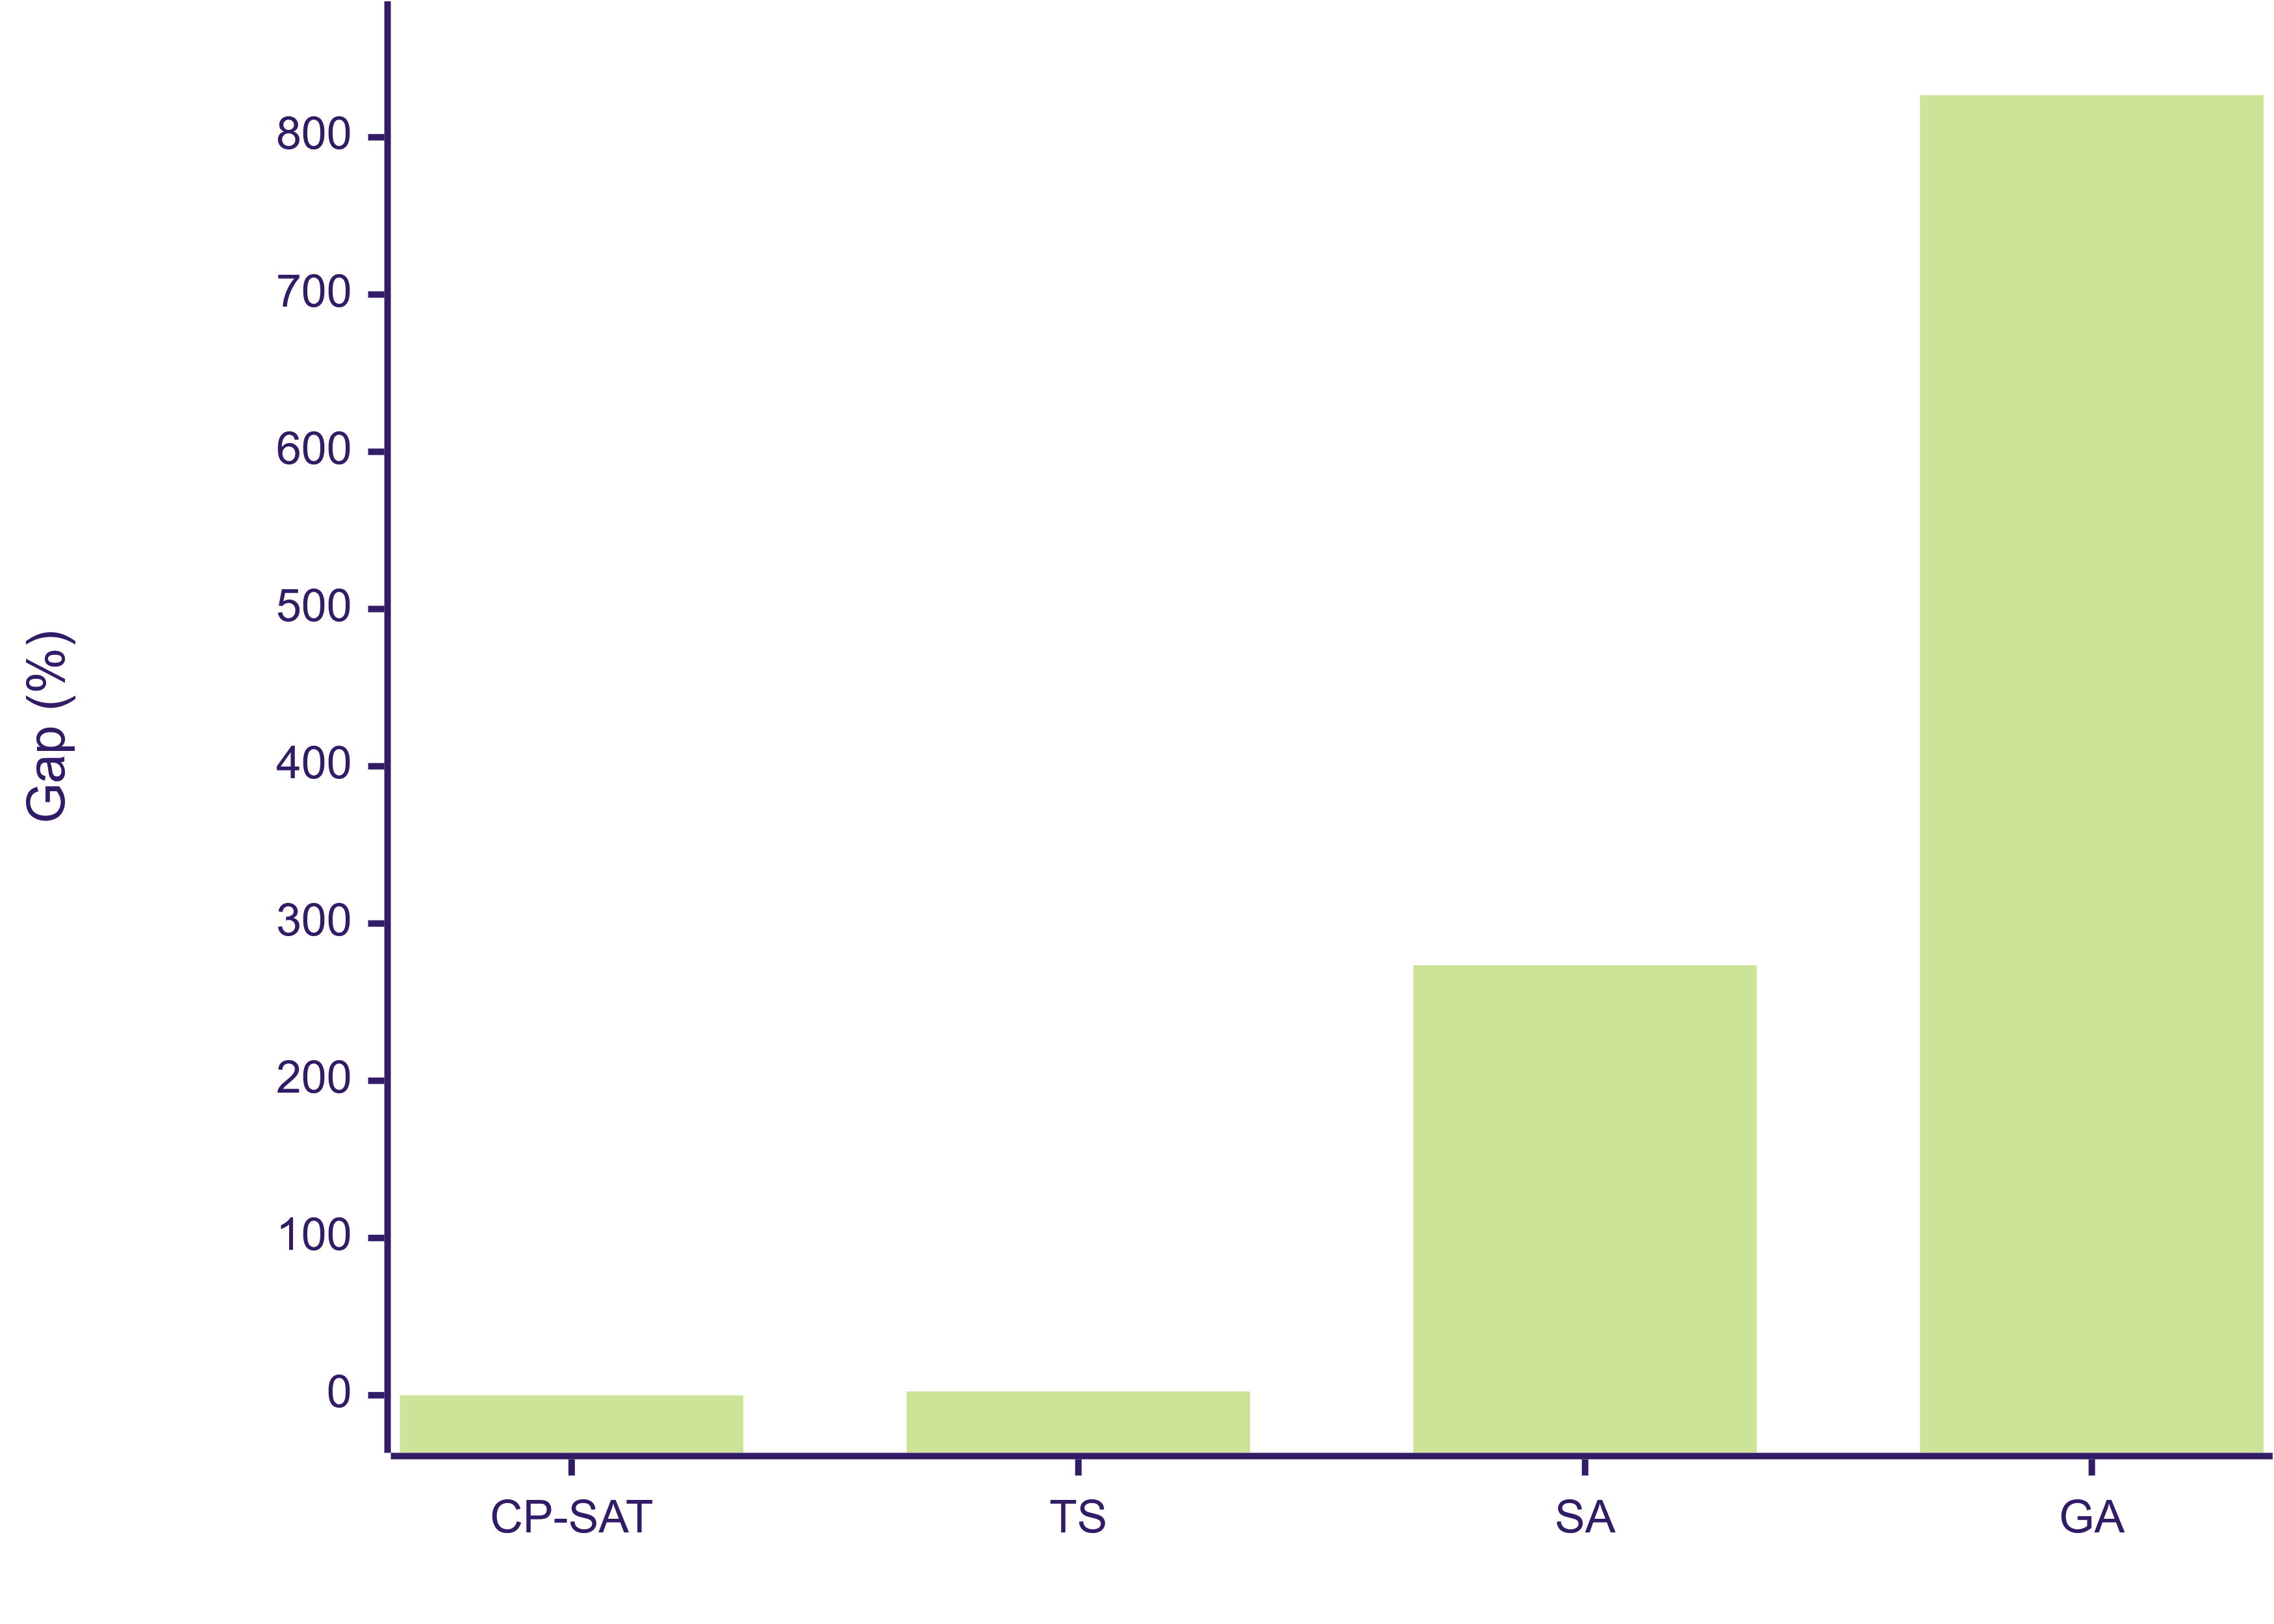
\includegraphics[width=0.8\textwidth]{images/Algorithms gap from the best.png}
    \caption{Отставание от оптимума (Gap, %)}
    \label{fig:AlgsGapPersent}
\end{figure}

\paragraph { Анализ компромисса: время выполнения и качество решения}

Мы сопоставили временные затраты алгоритмов с качеством итоговых расписаний (на примере датасета medium). Анализ данных позволяет сделать вывод о конкурентоспособности методов:

\begin{itemize}
\item Точность и эффективность: CP-SAT и метод поиска с запретами (TS) обеспечивают оптимальный баланс, находя решения с минимальным штрафом (~0.8) за доли секунды.
\item Скорость в ущерб качеству: Метод имитации отжига (SA) является наиболее быстрым, однако это ведет к снижению качества итогового расписания.
\item Ресурсная избыточность: Генетический алгоритм (GA) демонстрирует наиболее высокую вычислительную сложность при наихудших показателях качества среди исследованных методов.
\end{itemize}

\begin{figure}[h]
    \centering
    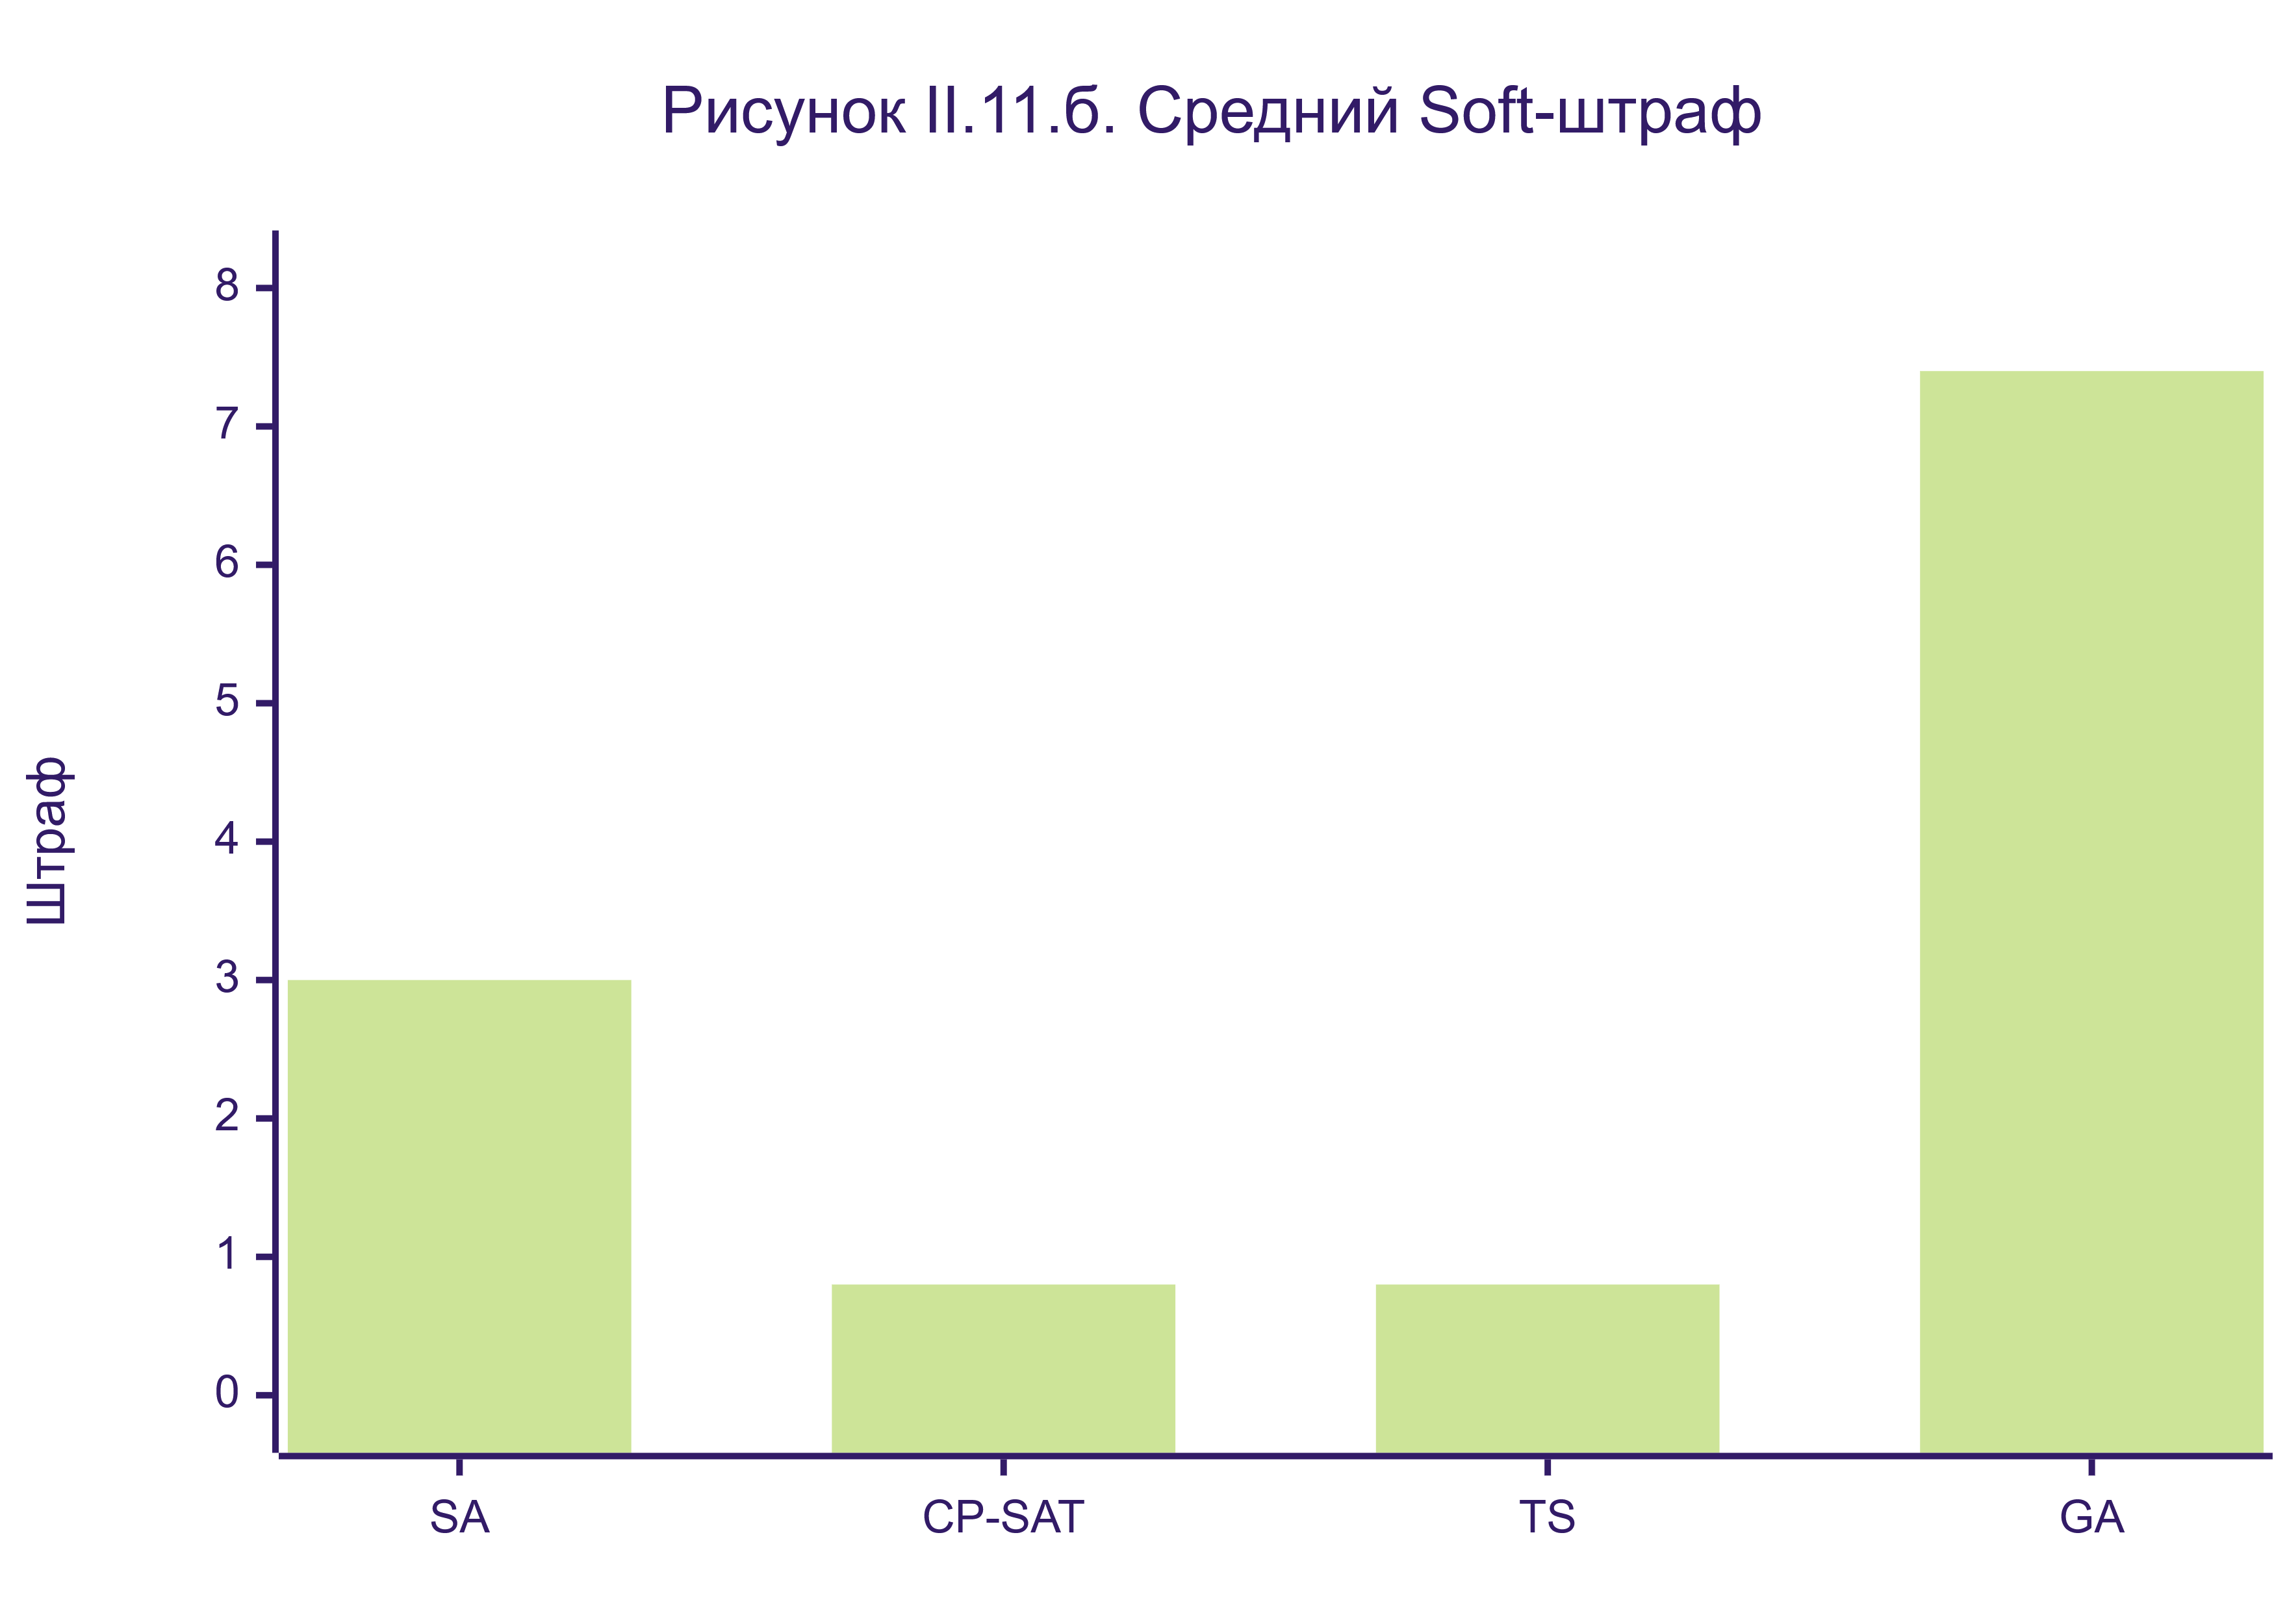
\includegraphics[width=0.8\textwidth]{images/Algorithms mean soft - medium.png}
    \caption{Средний Soft-штраф}
    \label{fig:AlgsmeanSoft}
\end{figure}

\subsubsection { Особый случай: структурно неразрешимый набор данных}

На наборе данных large_stress ни один из четырёх алгоритмов не нашёл допустимого решения, и для трёх эвристических методов число нарушений жёстких ограничений составило ровно двадцать четыре на каждом из десяти запусков без единого исключения — то есть совпало не приблизительно, а точно у всех трёх независимо реализованных методов. Решатель ограничений на этом же наборе данных строго доказал отсутствие допустимого решения вовсе. Поскольку ни одно из решений не является допустимым, сравнение по относительному отклонению от наилучшего найденного решения здесь неприменимо: имеет смысл сравнивать только сам остаточный штраф по мягким критериям при одинаковом, не сводимом к нулю числе жёстких нарушений, а также скорость, с которой каждый метод приходит к этому выводу.

\begin{table}[h]
\centering
\caption{Сравнение алгоритмов}
\label{tab:algorithms_comparison}
\begin{tabular}{lccc}
\hline
\textbf{Алгоритм} &
\textbf{Нарушений жёстких ограничений} &
\textbf{Среднее значение мягкого штрафа} &
\textbf{Среднее время, мс} \\
\hline
CP-SAT & доказано: решения не существует & --- & 13 \\
TS     & 24 & 0.028  & 828  \\
SA     & 24 & 3.676  & 148  \\
GA     & 24 & 11.148 & 6185 \\
\hline
\end{tabular}
\end{table}

\begin{figure}[h]
    \centering
    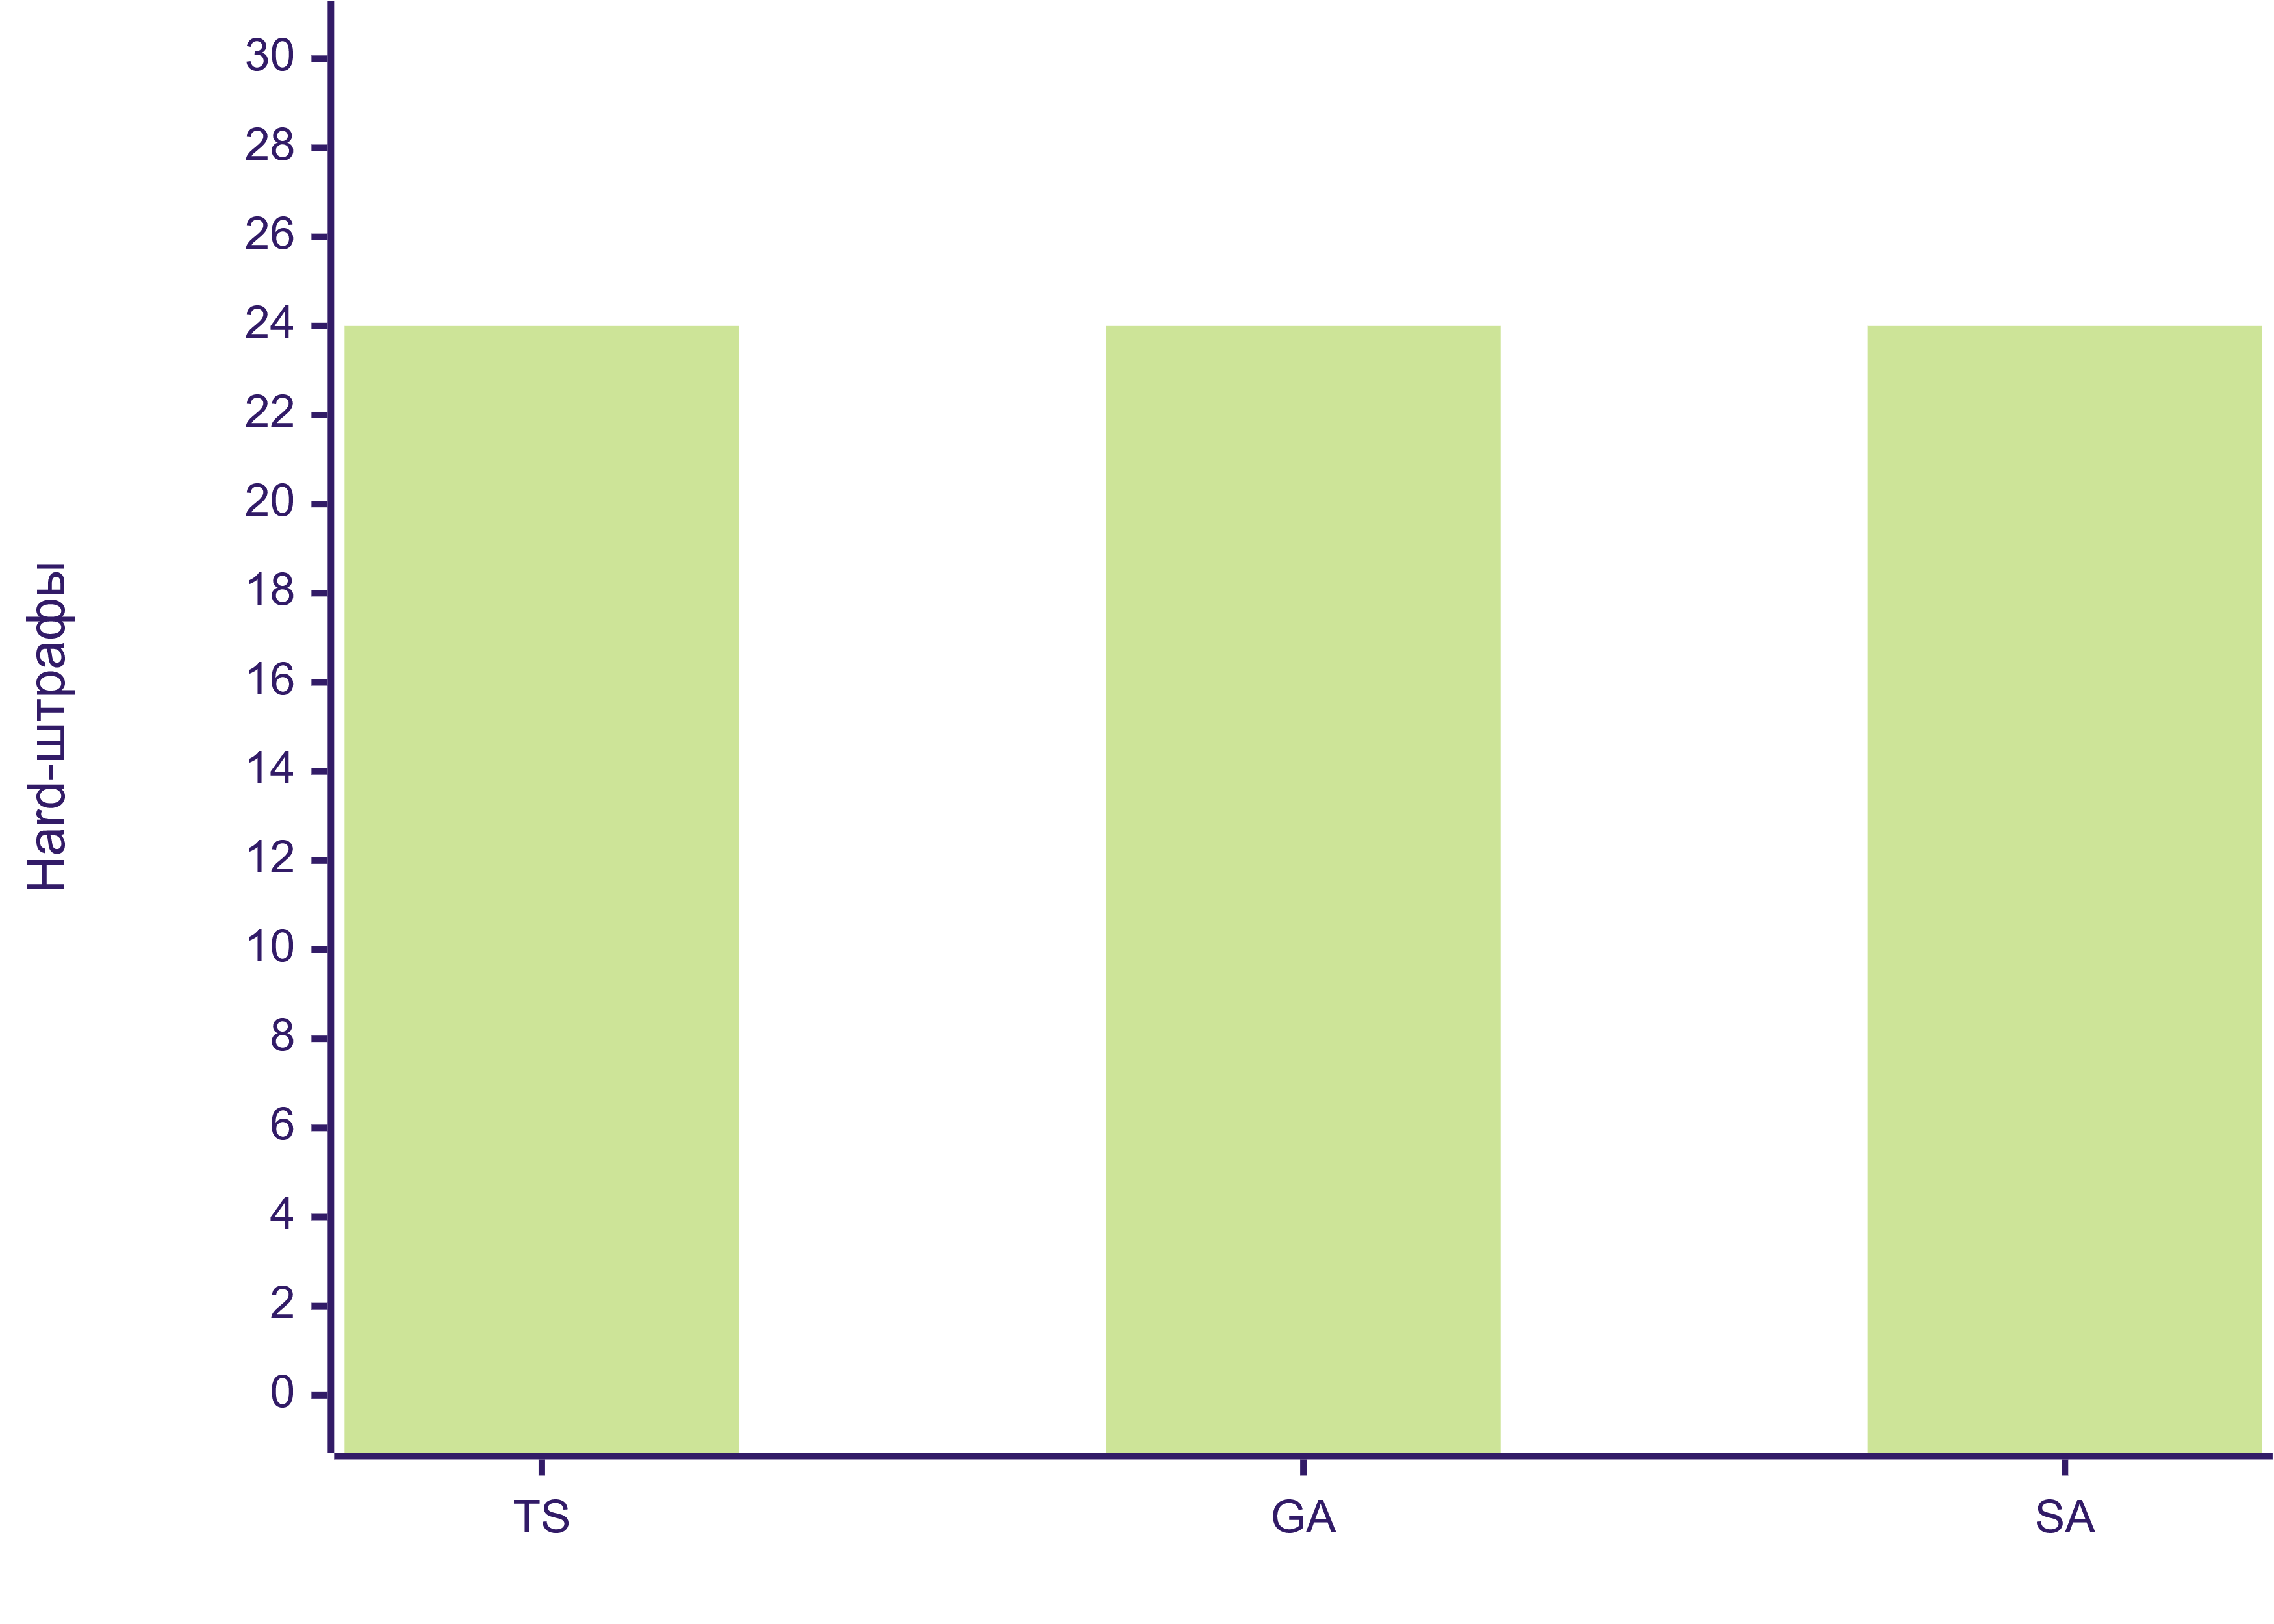
\includegraphics[width=0.8\textwidth]{images/Algorithms hard diif-large-stress.png}
    \caption{Сравнение нарушений hard-ограничений на датасете large_stress}
    \label{fig:AlgsHardDiffOnLargeStress}
\end{figure}

Совпадение числа жёстких нарушений у всех трёх эвристик — само по себе значимый результат: оно подтверждает, что структурный дефицит слотов (двадцать четыре занятия, для которых физически не нашлось свободного времени из пятидесяти четырёх) — объективное свойство самой задачи, а не особенность конкретного алгоритма или конкретного случайного запуска. При равном, неустранимом числе жёстких нарушений различие между методами проявляется только в том, насколько хорошо каждый из них распоряжается оставшейся свободой выбора среди тех решений, которые всё равно вынуждены нарушать ограничения: поиск с запретами заметно эффективнее минимизирует остаточный штраф по сравнению с имитацией отжига и тем более с генетическим алгоритмом, что согласуется с выводами, сделанными на разрешимых наборах данных в предыдущем разделе.

Скорость решателя ограничений на этом наборе данных заслуживает отдельного комментария: тринадцать миллисекунд — это не оптимизация полного решения, а доказательство его отсутствия, для которого решателю достаточно вывести логическое противоречие из ограничений, не перебирая варианты значений переменных вовсе. Это самое наглядное практическое проявление фундаментального различия между точным методом и метаэвристиками, обсуждавшегося в разделе II.4: эвристические методы тратят сотни миллисекунд или секунды, пытаясь найти то, чего не существует, тогда как точный метод почти мгновенно доказывает, что искать нечего.

\subsubsection { Общие выводы по результатам сравнения}

Сопоставление всех четырёх алгоритмов на четырёх наборах данных разного размера и структуры позволяет сформулировать три практических вывода. Во-первых, решатель ограничений CP-SAT следует использовать там, где допустимый размер задачи позволяет получить ответ за приемлемое время: он либо находит доказанно оптимальное решение, либо доказанно сообщает об отсутствии решения, что недостижимо ни одним из трёх эвристических методов. Во-вторых, среди трёх метаэвристик поиск с запретами на всех использованных наборах данных показал наилучшее соотношение качества решения и затраченного времени, и может рассматриваться как основной эвристический метод для задач, на которые точное программирование ограничений не успевает ответить за разумное время. В-третьих, генетический алгоритм в реализованном виде — с прямым позиционным кодированием решения и недешёвой функцией оценки приспособленности — не оправдывает свою существенно более высокую вычислительную стоимость по сравнению с поиском с запретами и имитацией отжига ни на одном из использованных наборов данных, и его практическая ценность в рассматриваемой постановке задачи ограничена случаями, требующими специфической для популяционных методов устойчивости к структуре пространства решений, не проявившейся в проведённом эксперименте.


\clearpage
\section*{ЗАКЛЮЧЕНИЕ}
\addcontentsline{toc}{section}{ЗАКЛЮЧЕНИЕ}

В рамках данной работы была решена задача разработки и сравнительного анализа четырёх алгоритмов автоматического построения расписания учебных занятий, основанных на принципиально разных подходах к оптимизации: генетическом алгоритме, имитации отжига, поиске с запретами и точном программировании ограничений. Все четыре алгоритма были реализованы на единой модели данных, описывающей дисциплины, преподавателей, аудитории и группы, и оценивались единым критерием качества решения, различающим жёсткие ограничения, нарушение которых делает расписание физически нереализуемым, и мягкие ограничения, отражающие желательные, но не обязательные свойства расписания.

Поставленные во введении задачи были выполнены последовательно и в полном объёме. Изучение теоретических основ задачи составления расписания и существующих подходов к её решению позволило обоснованно выбрать четыре рассмотренных алгоритма как представителей принципиально разных алгоритмических парадигм — от точного метода, гарантирующего оптимальность или доказывающего отсутствие решения, до метаэвристик, жертвующих этой гарантией в пользу гибкости и масштабируемости. Единая модель данных и единый критерий оценки качества, спроектированные до начала реализации конкретных алгоритмов, оказались необходимым условием честного сравнения: без них результаты разных алгоритмов были бы выражены в несопоставимых единицах измерения. Реализация всех четырёх алгоритмов сопровождалась рядом содержательных трудностей, часть которых была обнаружена не на этапе проектирования, а эмпирически — в частности, дефект, связанный с ограничением размера итогового расписания, проявившийся одинаково в трёх из четырёх реализаций и обнаруженный благодаря логическому противоречию между ответом точного решателя и ответами эвристических методов на одном и том же наборе данных. Этот эпизод сам по себе стал практическим подтверждением одного из выводов работы: наличие в распоряжении точного метода ценно не только как самостоятельный инструмент решения задачи, но и как средство проверки корректности эвристических реализаций.

Экспериментальное сравнение на наборах данных разного размера и структурной сложности показало, что поиск с запретами обеспечивает наилучшее соотношение качества решения и затраченного вычислительного времени среди трёх эвристических методов, имитация отжига является самым быстрым методом при умеренном качестве решения, а генетический алгоритм в реализованном виде уступает обоим по качеству при существенно более высоких вычислительных затратах. Решатель ограничений на разрешимых наборах данных находил решение, не худшее, чем любой из эвристических методов, а на структурно неразрешимом наборе данных — единственный из четырёх алгоритмов дал не приближённый, а доказанный ответ.

Практическая значимость работы заключается в том, что предложенная методика сравнения — единая модель данных, единый критерий оценки качества, проверка на нескольких независимых осях (случайность запуска и структура исходных данных) — может быть использована как основа для выбора конкретного алгоритма при построении полноценной системы автоматизации расписания, в зависимости от ожидаемого размера задачи и доступного времени на вычисление. Для образовательного учреждения с умеренным числом дисциплин и групп предложенные результаты прямо указывают на целесообразность использования точного метода либо, при больших объёмах данных, поиска с запретами как наиболее сбалансированной альтернативы.

Направления дальнейшего развития работы включают устранение выявленной, но не успевшей проявиться в эксперименте архитектурной неточности табу-списка в поиске с запретами, переход от взвешенной суммы мягких критериев к строго лексикографической многоступенчатой оптимизации в решателе ограничений там, где это содержательно оправдано, а также расширение модели данных поддержкой нескольких групп с пересекающимися ресурсами — преподавателями и аудиториями, — что превратило бы задачу из однопоточной в полноценную многогруппную постановку, ближе соответствующую масштабу реального учебного заведения.


\clearpage
\phantomsection
\renewcommand{\bibname}{БИБЛИОГРАФИЯ}
\section*{БИБЛИОГРАФИЯ}
\addcontentsline{toc}{section}{БИБЛИОГРАФИЯ}
\bibitem{FedkinSchedulingMethods}
Федькин Е. М. \textit{Разработка моделей, методов и алгоритмов составления расписаний традиционного и дистанционного обучения в высших учебных заведениях}. Диссертация Phd, Восточно-Казахстанский технический университет им. Д. Серикбаева, 2023. URL:
\url{https://ektu.kz/files/research/DissertationCouncil/fedkin/%D0%94%D0%B8%D1%81%D1%81%D0%B5%D1%80%D1%82%D0%B0%D1%86%D0%B8%D1%8F_%D0%A4%D0%B5%D0%B4%D1%8C%D0%BA%D0%B8%D0%BD.pdf}.

\bibitem{AlGabriSchedulingReview}
Аль-Габри В. М. \textit{Обзор литературных источников по теме «Автоматизация составления расписания занятий и экзаменов в высших учебных заведениях»}. Вестник Донского государственного технического университета, 2017. URL:
\url{https://cyberleninka.ru/article/n/obzor-literaturnyh-istochnikov-po-teme-avtomatizatsiya-sostavleniya-raspisaniya-zanyatiy-i-ekzamenov-v-vysshih-uchebnyh-zavedeniyah}.

\bibitem{MerkushevSchedulingMath}
Меркушев Р. В., Четтыкбаев Р. К. \textit{Математический аппарат автоматизированного составления расписаний}. Вестник Казахстанско-Американского Свободного Университета, 2024. URL:
\url{https://www.vestnik-kafu.info/pdf/vestnik-2024-3.pdf#page=174}.

\bibitem{HochbaumDualApproximation}
Hochbaum D. S., Shmoys D. B. \textit{Using dual approximation algorithms for scheduling problems theoretical and practical results}. Journal of the ACM, 1987. URL:
\url{https://doi.org/10.1145/7531.7535}.

\bibitem{WangHybridGeneticTabu}
Wang L., et al. \textit{A hybrid genetic tabu search algorithm based on a multi-operation joint movement neighborhood structure for job shop scheduling problems}. Complex & Intelligent Systems, 2025. URL:
\url{https://link.springer.com/content/pdf/10.1007/s40747-025-02026-0.pdf}.

\bibitem{MangalampalliSimulatedAnnealing}
Mangalampalli S. S., et al. \textit{Priority-Aware Multi-Objective Task Scheduling in Fog Computing Using Simulated Annealing}. Sensors, 2025. URL:
\url{https://doi.org/10.3390/s25185744}.

\bibitem{LiTabuReinforcementLearning}
Li L., et al. \textit{Tabu Search with Reinforcement Learning for Location Problems}. MODSIM World, 2025. URL:
\url{http://www.modsimworld.org/papers/2025/MODSIM_2025_paper_20.pdf}.

\bibitem{KononovRealTimeScheduling}
Кононов Д. А., Фуругян М. Г. \textit{Планирование вычислений в системах реального времени: эффективные алгоритмы построения оптимальных расписаний}. Программные продукты и системы, 2025. URL:
\url{https://www.mais-journal.ru/jour/article/download/2001/1437}.

\bibitem{NizamovaAggregativeGenetic}
Низамова Г. Ф. \textit{Математическое и программное обеспечение составления расписания учебных занятий на основе агрегативных генетических алгоритмов}. Автореферат диссертации, Уфимский государственный авиационный технический университет, 2006. URL:
\url{https://aimfirst.ru/docs/science/diss/r_autoref-matematicheskoe-i-programmnoe-obespechenie-sostavleniya-raspisaniya-uchebnykh-zanyatii-na-os.pdf}.

\end{document}
